\documentclass[12pt, a4paper]{report}
\linespread{1.3}
\setlength{\parindent}{1.25cm}

\usepackage[top=3cm,left=3cm,right=2cm,bottom=2cm]{geometry}
\usepackage{indentfirst}
\usepackage{amsmath, amsthm, amsfonts, amssymb}

\usepackage{graphicx}
\usepackage{color}
\usepackage{multicol}
\usepackage[normalem]{ulem}
\usepackage{wrapfig}
\usepackage{caption}
\usepackage{fancybox}
\usepackage[pdfstartview=FitH]{hyperref}
\usepackage{subfigure}
\usepackage{acronym}
\usepackage[T1]{fontenc}		% Selecao de codigos de fonte.
\usepackage[utf8]{inputenc}
\usepackage[brazil]{babel}
\usepackage{pgfplots,pgfplotstable}   % pacote para uso do pgfplots

\pgfplotsset{compat=1.3}
\usepackage{tikz}
\usepackage{array}
\usepackage{longtable}
\usepackage{pdfpages}
\usepackage{tikz}
\usepackage{graphicx}
\usepackage{verbatim}
\usepackage{fullpage}
\usepackage{pgf-pie}
\usepackage{enumitem}   



\usepackage{natbib} % criação de linhas

%Includes "References" in the table of contents
\usepackage[nottoc]{tocbibind}

\graphicspath{{Figuras/}} % caminho padrao imagens
% ------ Remove nome capitulo da tag chapter ---------


\makeatletter
\def\@makechapterhead#1{%
  \vspace*{0\p@}%
  {\parindent \z@ \raggedright \normalfont
    \interlinepenalty\@M
    \Huge\bfseries  \thechapter.\quad #1\par\nobreak
    \vskip 30\p@
  }}
\makeatother
\begin{document}



%---------- CAPA -------------
\pagestyle{empty}
\begin{center}

\includegraphics[height=2.5cm]{Figuras/UFBA.jpg}
% \hspace{2cm}
% 
\includegraphics[height=2.5cm]{Figuras/IM.jpg}
\hspace{2cm}

\includegraphics[height=2.5cm]{Figuras/DCCUFBA.jpg}
\end{center}

\begin{center}
\sc{\large{Universidade Federal da Bahia}} \\
\sc{\large{Instituto de Computação}} \\
\sc{\large{Bacharelado em Sistemas de Informação}} \\
\sc{\small{Trabalho de Conclusão de Curso}} \\

\vspace{3.6cm}

\sc{\Large{Sistema Colaborativo de \\Avaliação
Docente}}

\vspace{4.5cm}

\sc{\Large{Kênia Arruda Guimarães}}

\vspace{6.0cm}
\textbf{Salvador - Bahia} \\
Dezembro de 2021
\end{center}


\thispagestyle{empty}

%---------- FOLHA DE ROSTO -------------
\newpage
\begin{center}
\sc{\Large{Sistema Colaborativo de \\Avaliação
Docente}}

\vspace{4cm}

\large{Kênia Arruda Guimarães}
\end{center}

\vspace{4cm}

\begin{flushright}
\begin{minipage}{8.6cm}
Trabalho de Conclusão de curso apresentado como requisito parcial para obtenção do título de Bacharel em Sistemas de Informação.

\vspace{0.5cm}
\textbf{Orientador}: Prof. Dr. Rodrigo Rocha Gomes e Souza.

\end{minipage}
\end{flushright}
 
\vspace{6.95cm}

\begin{center}
\textbf{Salvador - Bahia} \\
Dezembro de 2021
\end{center}
\thispagestyle{empty} 

%---------- BANCA EXAMINADORA -------------
\newpage
\begin{center}
\sc{\Large{\textbf{Termo De Aprovação}}}
\vspace{1.3 cm}
\par\sc{\Large{Sistema Colaborativo de \\Avaliação Docente}}

\vspace{2cm}

\large{Kênia Arruda Guimarães}
\end{center}

\vspace{1.3 cm}

\begin{flushright}
\begin{minipage}{8.6cm} 
Trabalho de Conclusão de curso apresentado como requisito parcial para obtenção do título de Bacharel em Sistemas de Informação.
\end{minipage}
\end{flushright}
 
\vspace{1.5cm}
\begin{center}
\Large \textbf{Banca Examinadora:}
\end{center}
\vspace{1cm}

\begin{flushright}
\begin{minipage}[l]{12cm}
\begin{center}
\uline{\hspace{10.5cm}} \\
Prof. Dr. Rodrigo Rocha Gomes e Souza (Orientador) \\ Universidade Federal da Bahia \\
\vspace{1cm}
\uline{\hspace{10.5cm}} \\
Profª. Drª Christina von Flach Garcia Chavez\\ Universidade Federal da Bahia \\
\vspace{1cm}
\uline{\hspace{10.5cm}} \\
Profª. Drª Tatiane Nogueira Rios\\ Universidade Federal da Bahia \\


\end{center}
\end{minipage}
\end{flushright}
\thispagestyle{empty} 

%-----------Dedicatória----------------
\newpage
\vspace*{21.9cm}
\begin{flushright}
\textit{Dedico este trabalho à minha família}
\end{flushright}
\thispagestyle{empty} 


%------------Agradecimentos------------
\newpage
\chapter*{Agradecimentos}
\thispagestyle{empty}
Aos meus pais, que sempre estiveram ao meu lado me apoiando em cada decisão tomada.

À minha noiva, Juliana Alves Pereira, que vem sendo meu maior suporte e incentivo neste ciclo de aprendizado. 

Aos meus amigos e em especial à Lina Mendes, que me deu grande auxílio no design da aplicação, ao Carlos Henrique e Ludmila Cruz, que sempre tiveram muita paciência ao ouvir os desabafos quando ainda não tinha encontrado a solução para alguns dos obstáculos que encontrei durante a a execução deste projeto, e em memória a Erick Vian, que sempre foi meu grande incentivador na conclusão deste curso e hoje sei que está torcendo por mim lá de cima.

Ao meu orientador Rodrigo Rocha Gomes e Souza, pela excelente orientação, paciência e atenção prestados no desenvolvimento deste trabalho, e à Universidade Federal da Bahia (UFBA), pelo espaço público de ensino que, mesmo com todas as dificuldades encontradas, forma excelentes profissionais que vêm contribuindo constantemente para o desenvolvimento do nosso país.  

\thispagestyle{empty} 
%------------Citação-------------------
\newpage
\vspace*{20cm}
\begin{flushright}
\begin{minipage}{8cm}
\begin{flushright}
\textit{
``Toda a ciência é nada mais do que um refinamento do pensamento cotidiano''. \\
Albert Einstein}
\end{flushright}
\end{minipage}
\end{flushright}
\thispagestyle{empty} 

%--------------Resumo-------------------
\newpage
\chapter*{Resumo}
Na Universidade Federal da Bahia \ac{UFBA}, a avaliação docente é realizada semestralmente pelos alunos através de uma ferramenta considerada pelos mesmos como de propósito raso e sem transparência, causando sentimento de insatisfação. 

Nesse contexto foi desenvolvida a solução Sistema Colaborativo de Avaliação Docente, ou SICAD, que é um sistema web que tem por objetivo a avaliação dos docentes da \ac{UFBA} de forma paralela com o instrumento avaliativo já utilizado por esta. Através do compartilhamento das experiências vividas em sala de aula pelos discentes, assim como um processo de avaliação individual do docente, é possível gerar resultados que podem servir de subsídio para tomadas de decisão no processo de matrícula por parte dos discentes e pelos colegiados no que diz respeito à indicação de disciplinas aos docentes.

Este trabalho contém  uma avaliação realizada considerando a  aplicação final disponibilizada à comunidade acadêmica, avaliando os objetivos de usabilidade das principais funcionalidades que nele foram desenvolvidas.

Como resultado da avaliação temos que as funcionalidades da solução \ac{SICAD} geram sentimento de satisfação aos seus usuários, ou seja, cumpriram seu objetivo proposto e agregam valor principalmente na avaliação docente.

\textbf{Palavras-chave:} <Avaliação Docente>, <Universidade Federal da Bahia>, <Comunidade Acadêmica>, <SICAD>.
\thispagestyle{empty} 

%-------------Abstract------------------
\newpage
\chapter*{Abstract}
At the Federal University of Bahia \ac{UFBA}, teacher assessment is carried out every six months by students using a tool considered by them poor in purpose and without transparency, causing a feeling of dissatisfaction.

In this context, the Collaborative System for Teacher Assessment, or SICAD, was developed, which is a web system that aims to assess the teachers at \ac{UFBA} in parallel with the assessment tool already used by it. Through the sharing of experiences lived in the classroom by the students, as well as an individual evaluation process of the teacher, it is possible to generate results that can serve as a subsidy for decision-making in the enrollment process by the students and by the collegiate bodies with regard to indication of subjects to teachers.

This work contains an evaluation carried out considering the final application made available to the academic community, evaluating the usability goals of the main features that were developed in it.

As a result of the evaluation, the features of the \ac{SICAD} solution generate a feeling of satisfaction to its users, that is, they have fulfilled their proposed objective and add value mainly to the teacher's evaluation. 

\textbf{Key words:} <Teacher Evaluation>, <Federal University of Bahia>, <Academic Community>, <SICAD>.
\thispagestyle{empty} 

% ----------- Lista de figuras ----------

\pdfbookmark[0]{\listfigurename}{lof}
\listoffigures
\cleardoublepage

%--------- Lista de tabelas ---------

\pdfbookmark[0]{\listtablename}{lot}
\listoftables
\cleardoublepage

%-------------Índice--------------------
\newpage
\tableofcontents
\thispagestyle{empty}


%--------- Lista de Siglas---------
\chapter*{Lista de Siglas}
\addcontentsline{toc}{chapter}{Lista de Siglas} 

\begin{acronym}
\acro{SICAD}{Sistema Colaborativo de Avaliação Docente}
\acro{SIAV}{Sistema de Avaliação Docente}
\acro{UFBA}{Universidade Federal da Bahia}
\acro{SUPAC}{Superintendência de Administração Acadêmica}
\acro{IES}{Instituições de Ensino Superior}
\acro{SIGAA}{Sistema Integrado de Gestão de Atividades}
\acro{CAD}{Comissão de Atividades Docentes}
\acro{IME}{Instituto de Matemática e Estatística}
\acro{SINAES}{Sistema Nacional de Avaliação da Educação Superior}
\acro{CPA}{Comissão Própria de Avaliação}
\acro{RBAC}{Role Based Access Control}
\acro{HBS}{Hash Based Signature}
\end{acronym}

\chapter{Introdução}
\label{chap:introducao}

Na Universidade Federal da Bahia(\ac{UFBA}), atualmente, a avaliação docente é realizada através do Sistema de Avaliação Docente, SIAV\footnote{Disponível em \url{http://www.siav.ufba.br/}.} Semestralmente, os alunos participam deste processo, respondendo a um questionário de acordo com os objetivos dispostos na aplicação. No entanto, a  ferramenta disponibilizada é obsoleta, não possuindo uma versão mais atualizada que demonstre os resultados de forma mais transparente, resumida e atrativa para a comunidade acadêmica.

Através de diálogo com estudantes e contato com redes sociais utilizadas pelos mesmos, foi possível mapear falhas, críticas e sugestões em torno do processo  avaliativo realizado através do SIAV na \ac{UFBA}.

Focado na exibição dos resultados das avaliações e comentários construtivos, surge o Sistema Colaborativo de Avaliação dos Docentes(\ac{SICAD}), uma aplicação web que permite aos discentes da instituição UFBA realizarem avaliações docentes de forma mais simples e rápida, realizarem comentários construtivos sobre disciplinas cursadas e visualizarem os resultados de forma mais efetiva.

Para realização do desenvolvimento desta aplicação, foi feito um estudo teórico sobre processamento de linguagem natural com o propósito de subsidiar a construção de um algoritmo que encorajasse a realização de um comentário construtivo dentro do sistema. Outro ponto focal na aquisição de conhecimento foi o estudo realizado sobre \textit{crawlers}, que serviram no entendimento para adaptação de uma rotina utilizada na obtenção de dados consumidos pela ferramenta assim como a segurança da informação também foi explorada, trazendo conceitos de \textit{hash} para tratamento de informações sensíveis dentro a aplicação. Por fim, trabalhos relacionados também foram utilizados como forma de conhecimento e contribuíram no desenvolvimento do \ac{SICAD}.

Para avaliar a satisfação na utilização do \ac{SICAD}, foi elaborada uma pesquisa e disponibilizada aos usuários através do Google Forms, com objetivo centrado na usabilidade e facilidade da utilização da aplicação. A pesquisa demostrou um resultado positivo, ou seja, a ferramenta alcançou seu objetivo proposto.

Os capítulos desta monografia estão organizados de tal maneira: o Capítulo 2 apresenta informações sobre o domínio acadêmico, conceitos utilizados no desenvolvimento da aplicação, como processamento de linguagem natural referenciando a técnica de pré-processamentos stemming, extração de dados utilizando a técnica crawler, segurança da informação com explanação sobre algoritmos hash utilizado no tratamento de informação sensíveis dentro da aplicação, além de uma lista de trabalhos trabalhos relacionados que foram feitos por universidades com o propósito de avaliação docente. No Capítulo 3 são apresentados os principais aspectos da aplicação desenvolvida, incluindo a contextualização de conceitos e suas funcionalidades. O Capítulo 4 traz uma avaliação da usabilidade relacionada aos objetivos da aplicação. Por fim, o Capítulo 5 apresenta a conclusão desta monografia, trabalhos futuros e as considerações finais.


\chapter{Fundamentação Teórica}
\label{chap:fundamentacaoteorica}

Neste capítulo serão abordadas conceitos utilizados na construção da aplicação \ac{SICAD}. Para o desenvolvimento deste trabalho foi utilizado processamento de linguagem natural para reconhecimento de padrões através da técnica \textit{stemming}. Na área de extração de dados será abordado o
conceito de \textit{crawler} tal qual foi utilizado para coletar as informações sobre disciplinas e docentes da universidade que serão utilizadas nas avaliações realizados pelos discentes. É apresentada uma seção abordando os algoritmos de segurança utilizados pela aplicação e a seguir são abordados os trabalhos relacionados que foram estudados e utilizados para desenvolvimento do aplicativo web.

\section{Processamento de Linguagem Natural}

Segundo \cite{chowdhury2003}, processamento de linguagem natural é uma área de pesquisa e de aplicação que explora como os computadores podem ser usados para processar e manipular texto ou discurso em linguagem natural para fazer coisas úteis. Com essa tecnologia, os computadores podem ser treinados para cumprir tarefas específicas ao processar grandes quantidades de dados e reconhecer padrões nesses dados.
Este trabalho utiliza o conceito de \textit{stemming} para reconhecer radicais de palavras de baixo calão utilizadas na seção de comentários construtivos da aplicação e será abordado a seguir.

\subsection{Stemming}
 \emph{Stemming} é o processo de conflação\footnote{O termo conflação está empregado no lugar de \emph{conflation} em inglês por não haver uma boa tradução para o português. Entende-se por conflação onde dois ou mais termos são utilizados indistintamente para uma determinada finalidade, conforme Freund (1982).} onde há diferentes formas de uma palavra em uma única representação.
A palavra raiz, base ou forma raiz resultante do processo de reduzir as palavras flexionadas (ou, às vezes, derivadas) não precisa ser idêntico à raiz morfológica da palavra; geralmente é suficiente que as palavras relacionadas mapeiem o mesmo radical, mesmo que esse radical não seja, em si, uma raiz válida.

Existem diversas técnicas para realizar o processo de stemming, como o uso de dicionários e variedade de sucessores. Contudo, a técnica mais comum é a remoção de afixos da palavra. Essa técnica retira prefixos e/ou sufixos das palavras através da aplicação sucessiva de um conjunto regras até chegar ao \emph{stem} resultante, ou seja, a raiz. Neste trabalho, os \emph{stemmers} usam a técnica de remoção de afixos para chegar a uma raiz que será buscada em uma base de dados contendo palavras de baixo calão.   

\section{Extração de Dados}
Para captura das informações deste trabalho foi utilizado um \textit{crawler} responsável por coletar as informações para serem armazenadas em banco de dados e utilizadas pela aplicação.

\subsection{Crawler}
Para \cite[p. 1]{ilprints376}, em tradução livre, um crawler é \textit{"uma coleta automática de páginas da web para criar um índice local e/ou local de coleção de páginas da web."}, ou seja, um programa ou \textit{script} que percorre e que coleta informação em páginas da internet, podendo criar índices e/ou armazenar esses dados bem como atualizá-los. 

Neste trabalho foi aperfeiçoado um algoritmo que realiza  a identificação das disciplinas dos cursos Ciência da Computação, Engenharia da Computação, Sistemas de Informação e Licenciatura em Computação da UFBA, assim como os discentes que as ministram, e persiste essas informações em um banco de dados para serem consumidas pela aplicação posteriormente nos módulos de comentários e avaliação.

\section{ Segurança}
\label{sec:seguranca}

O controle sobre uma informação é observado na aplicação de alguns fundamentos, também chamados de “pilares da segurança da informação". A \cite{iso27001} descreve em suas primeiras linhas alguns desses pilares:

\textit{“O sistema de gestão da segurança da informação preserva a confidencialidade, integridade e disponibilidade da informação por meio da aplicação de um processo de gestão de riscos e fornece confiança para as partes interessadas de que os riscos são adequadamente gerenciados.”}

Estabelecida em 2013, essa visão apresenta três fundamentos básicos: confidencialidade, integridade e disponibilidade, e para este trabalho serão considerados os mesmos. Percebemos que os três pilares podem auxiliar muito no manuseio das informações. Eles são a base para a construção de sistemas e garantem sua proteção. A seguir, uma descrição das principais características de cada fundamento. Vale lembrar que a segurança da informação não se limita à informação digital, pois todos os princípios se aplicam também à informação em meio físico (arquivos, formulários, documentos, etc.).
\begin{itemize}
\item Confidencialidade: Manter a informação indisponível a todos, exceto de quem é autorizado a vê-la.
\item Integridade: Assegurar que a informação não foi alterada por meios desconhecidos ou não autorizados.
\item Disponibilidade: Garantir acesso à informação e os ativos sempre que necessário.
\end{itemize}

Neste trabalho foram considerados os três fundamentos apresentados que serão referenciados nos próximos tópicos deste trabalho. A seguir no subtópico \ref{subsec:hash} será explanado um pouco sobre o conceito de Hashing e como esse algoritmo foi utilizado para manter o pilar da integridade da informação.

\subsection{Hashing}
\label{subsec:hash}
As funções hash criptográficas ou funções de resumo (em inglês, hash) de forma simplificada são algoritmos complexos que transformam uma quantidade de informações em uma saída de comprimento fixo. O processo é feito através do uso de fórmulas matemáticas e é interessante o uso de um computador para ser alcançado de forma mais ágil. Contudo, o mesmo poder ser realizado de forma manual.

As chamadas Hash Based Signatures (HBS) foram propostas inicialmente por \cite{lamport1979constructing}. Basicamente pra se obter um hash é preciso uma string de entrada  que gerará uma sequência de letras e números aleatórios Conhecida como a impressão digital, toda vez que a string de entrada é modificada sua impressão digital também é alterada.

Normalmente, os algoritmos de hashing  são projetados como funções de sentido único, o que significa que elas não podem ser facilmente revertidas sem empregar grandes quantidades de tempo e de recursos computacionais. Em outras palavras, é muito fácil criar o output a partir do input, mas relativamente difícil de ir na direção oposta (gerar o input a partir do output apenas). De um modo geral, quanto mais difícil for de encontrar o input, mais seguro será o algoritmo de hashing.

Segundo o que foi explanado sobre integridade podemos perceber que ser ela pode ser implementada utilizando mecanismos de segurança, como criptografia e hashing.

Na segurança da informação funções hash podem ter varias aplicabilidades principalmente em assinatura digital, código de autenticação de mensagem (MACs), e formas de autenticação. 

Existem vários tipos diferentes de funções hash, contudo, para este trabalho vamos considerar a função hash criptográfica SHA-2 sob a variação de 256 bits, conhecida como SHA256 que será explorada no subtópico \ref{subsec:sha256}.

\subsection{SHA-256}
\label{subsec:sha256}

O Secure Hash Algorithm (SHA) foi desenvolvido em 1994 pelo National Institute of Standards and Technology (NIST) junto com National Security Agency (NSA), ambas agências mantidas pelo governo dos Estados Unidos, para ser usado como padrão.

A primeira versão, SHA-0, foi publicada em 1993, com uma impressão digital de 160 bits. Em 1995, foi publicada SHA-1, que é muito parecida com sua antecedente, alterando a especificação de dispersão do SHA-0 e corrigindo possíveis fraquezas. SHA-2 foi publicada em 2001, e é significantemente diferente da função de dispersão SHA-1; sua impressão digital pode ser dada em 224, 256, 384 ou 512 bits. Em 2012 o NIST selecionou um algoritmo adicional, o Keccak, para padronização sob o título de SHA-3.

Diferentes funções hash produzirão outputs de tamanhos diferentes, mas os possíveis tamanhos de output para cada algoritmo de hashing são sempre constantes. Por exemplo, o algoritmo SHA-256 só pode produzir outputs de 256 bits, enquanto o SHA-1 irá sempre gerar um hash de 160 bits.

Exemplificando, vamos utilizar os seguintes usernames fictícios “maria” e “Maria”. Executando o algoritmo hash SHA-256 iremos obter os resultados descritos na tabela \ref{tab:sha256}.

\begin{table}[ht!]
\begin{tabular} { |p{1cm}|p{15.5cm}|  }
 \hline
 \multicolumn{2}{|c|}{SHA-256} \\
 \hline
Input & Output(256 bits) \\
 \hline
 maria & 94AEC9FBED989ECE189A7E172C9CF41669050495152BC4C1DBF2A38D7FD85627 \\
 Maria&  9FF18EBE7449349F358E3AF0B57CF7A032C1C6B2272CB2656FF85EB112232F16  \\
 \hline

\end{tabular}
 \caption{Demonstração do uso do SHA-256}
\label{tab:sha256}
\end{table}

Note que uma pequena alteração (na primeira letra maiúscula) resultou em um valor de hash totalmente diferente. Mas como estamos usando o SHA-256, os outputs sempre terão um tamanho fixo de 256 bits (ou 64 caracteres) independentemente do tamanho do input. Além disso, não importa quantas vezes executamos as duas palavras através do algoritmo, os dois outputs permanecerão constantes.

Neste trabalho foi escolhido a variação de 256 bits da SHA-2 porque ela é considerada segura e nos retorna uma impressão digital com tamanho suficiente pra representar os usuários do sistema. 

\subsection{Salt}

O salt é uma string aleatória que pode ser concatenada (préfixando ou pós-fixando) a informação onde é aplicada um hash. Adicionar um salt aleatório garante que o hash produzido será sempre diferente dando uma camada extra de proteção para a informação.

Uma regra utilizada de forma comum é usar um salt grande e complexo, do tamanho da saída da função hash, ou seja, utilizando um hash SHA256, o salt deve ter 256 bits aleatórios.

Para este trabalho foi gerado um salt de 256 bist, aplicado um hash SHA256 nesse mesmo salt e por fim concatenado ao username. POr conseguinte,  aplicado novamente um hash SHA256 para garantir segurança extra no usuário do sistema.

\chapter{Trabalhos Relacionados}
\label{chap:trabalhorelacionados}

Para desenvolvimento deste trabalho foram pesquisados e estudados projetos relacionados com a proposta inicial introduzida no capítulo introdutório. Foram levantadas propostas fora do país e dentro do território brasileiro a fim de subsidiar abordagens diferentes para a concepção da solução proposta.
\subsection{RateMyProfessors}
O RateMyProfessors \footnote{RateMyProfessors. Disponível em <\url{www.ratemyprofessors.com}>. Acesso em: 17 nov. 2019.} é um site de avaliação docente, concebido em maio de 1999 por John Swapceinski. Inicialmente o site foi lançado como TeacherRatings e mais tarde, no ano de 2001, passou a se chamar RateMyProfessors. O sistema permite que os discente de universidades atribuam classificações a docentes de instituições americanas, canadenses e do Reino Unido.

A plataforma tem como foco a avaliação de professores utilizando conceitos como nível de dificuldade, atribuições de \textit{tags} (palavras-chave), como por exemplo "respeitoso", "faz muitos artigos", "atividades para casa", bem como um comentário de até 350 caracteres ao final de cada avaliação. É possível cadastrar professores caso eles não estejam na base de dados e os comentários e avaliações são anônimos.

Para ser publicado, o usuário deve estar autenticado e classificar o curso e/ou professor em uma escala de barra de 1 a 5 nas seguintes categorias: "qualidade geral" e "nível de dificuldade". O avaliador também pode compartilhar se eles cursariam a disciplina com o professor novamente, se a participação na aula é obrigatória, se utiliza a bibliografia indicada, entre outros. Os avaliadores também podem selecionar até três \textit{tags} que descrevem o professor de uma lista de 20 que é disponibilizada. Na Figura \ref{fig:ratemyprofessor} visualizamos a inserção de uma avaliação docente.
\begin{figure}
\centering
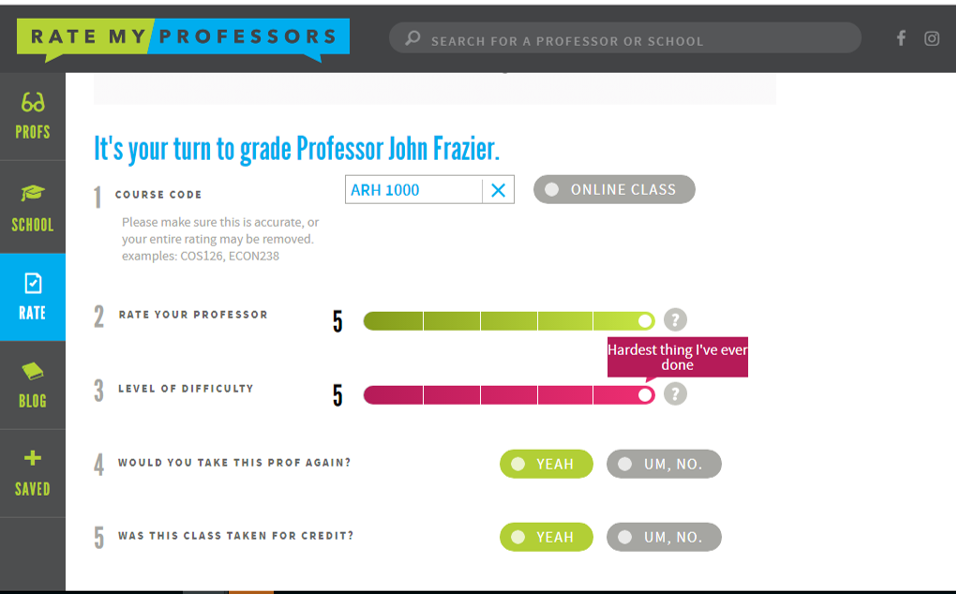
\includegraphics[scale=0.45]{ratemyprofessor.png}
\caption{Processo de Avaliação Docente do site RateMyProfessors.}
\label{fig:ratemyprofessor}
\end{figure}

Dentre as funções existentes, é importante destacar a avaliação das disciplinas dos docentes, pois é um recurso que se assemelha ao desenvolvido no SICAD.

\subsection{RateMyTeachers}

O RateMyTeachers\footnote{RateMyTeachers. Disponível em <\url{www.ratemyteachers.com/}>. Acesso em: 17 nov. 2019.}, assim como o RateMyProfessor, é um site de avaliação docente, porém seu objetivo é a classificação de professores de ensino fundamental e médio e escolas. Os usuários podem classificar seus professores em uma escala de 1 a 5 nas categorias facilidade, utilidade, conhecimento e clareza ao passar o conhecimento, com os dois últimos considerando uma pontuação de "qualidade geral". É permitido realizar comentários sobre as experiências com os professores.

O site foi lançado em 2001 pela Mister Message e posteriormente vendido ao ex-proprietário Patrick Nagle. Atualmente o site atende instituições de ensino nos Estados Unidos, Reino Unido, Canadá, Irlanda, Austrália e Nova Zelândia.

Um fato pertinente referente ao RateMyTeachers é que inicialmente o mesmo era moderado por uma comunidade pública de voluntários. Esta comunidade pública foi substituída em 2017 por uma comissão de moderação privada que se encarrega de revisar manualmente todas as classificações e professores adicionados ao site. 
Podemos observar na Figura \ref{fig:ratemyteacher} o processo inicial de inserção de uma avaliação docente.

\begin{figure}
\centering
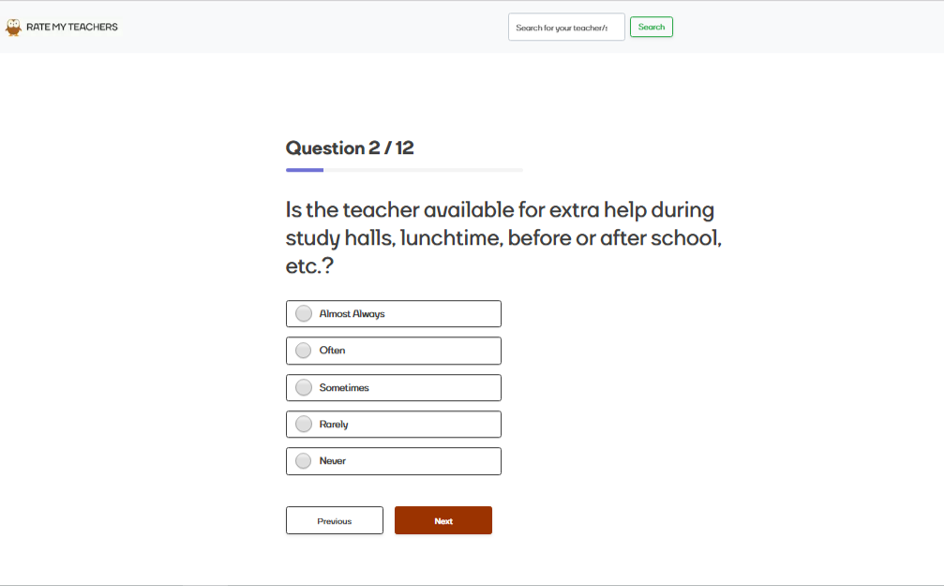
\includegraphics[scale=0.45]{ratemyteachers.png}
\caption{Processo de Avaliação Docente do site RateMyTeachers.}
\label{fig:ratemyteacher}
\end{figure}

Dentre as funcionalidades citadas no RateMyTeachers, evidencia-se a  avaliação docente e realização dos comentários, propósitos também disponíveis no SICAD.

Após pesquisa não foram encontradas plataformas nacionais com a finalidade de avaliação docente de alcance nacional e internacional como o RateMyProfessor e o RateMyTeachers respectiavemente.

\subsection{Avaliação Docente nas Instituições de Ensino Superior}

 A Lei Federal nº 10.861, de 14 de abril de 2004, instituiu o Sistema Nacional de Avaliação da Educação Superior (SINAES), prevendo que toda instituição de ensino superior (IES), pública ou privada, deverá constituir uma Comissão Própria de Avaliação (CPA), que será responsável pela autoavaliação da instituição. O SINAES avalia aspectos que giram em torno de alguns eixos principais definidos. São eles o ensino, a responsabilidade social, a pesquisa, a extensão, a gestão da instituição, o desempenho dos alunos, as instalações e o corpo docente.
 Toda instituição deverá realizar o levantamento de informações referentes à avaliação institucional. Cada \ac{IES} forma sua \ac{CPA} e nela define os instrumentos de coleta de dados tais como formulários, pesquisas online, sistemas de informações gerais (SIG) e etc. 
 
 \subsubsection{Universidade Federal da Bahia}
A UFBA realiza a avaliação docente através do Sistema de Avaliação Docente pelo Discente, o \ac{SIAV}, para todos os cursos de graduação e o Sistema Integrado de Gestão de Atividades Acadêmicas, \ac{SIGAA}, para os cursos de pós-graduação, onde é envolvida a comunidade acadêmica (docentes, discentes e coordenadores).

O atual instrumento avaliativo apresenta-se na forma de um questionário online que possui perguntas fechadas com múltiplas opções de resposta como concordo totalmente, concordo parcialmente,Não concordo/nem discordo,discordo parcialmente e discordo totalmente. Os discentes ao respondê-lo avaliam diferentes aspectos que se referem competência técnica, relacional e didática assim como o compromisso do professor em cumprir os requisitos do planejamento apresentado no inicio do semestre. Há também uma autoavaliação disponível para o aluno onde ele avalia sua participação nos componentes curriculares cursados.

Este processo avaliativo é realizado ao final de cada semestre e é pré-requisito para liberação da matricula web, ou seja, é obrigatório para discentes a partir do 2º semestre na universidade.

Nas figuras \ref{fig:siav_tela} e \ref{fig:siav_avalia} observamos a tela inicial e avaliação docente respectivamente no sistema SIAV.

\begin{figure}
\centering
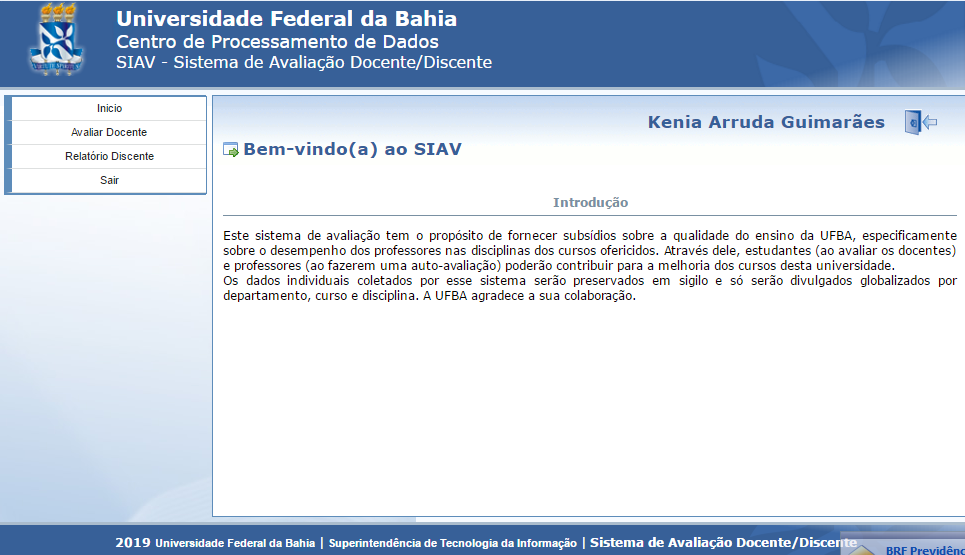
\includegraphics[scale=0.6]{siav_tela_inicial.png}
\caption{Tela Inicial do SIAV}
\label{fig:siav_tela}
\end{figure}

\begin{figure}
\centering
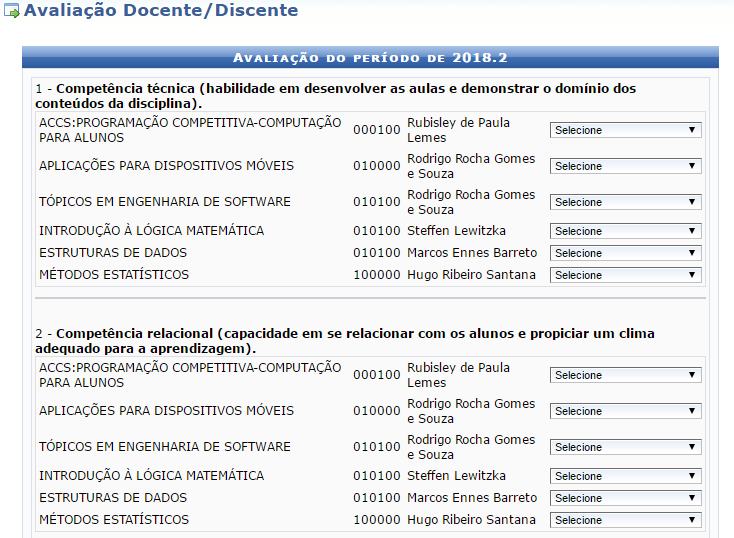
\includegraphics[scale=0.6]{siav_avaliacao.png}
\caption{Tela de Avaliação Docente do SIAV}
\label{fig:siav_avalia}
\end{figure}

\subsubsection{Universidade de Brasília}
Chamado de Avaliação Discente \footnote{Avaliação Discente. Disponível em <\url{www.cpa.unb.br}>. Acesso em: 18 nov. 2019.}, o processo realizado pela Universidade de Brasília (UNB) é realizada no início de todo semestre através da plataforma de matrícula online (MatriculaWeb)\footnote{MatriculaWeb. Disponível em <\url{www.matriculaweb.unb.br}>. Acesso em: 18 nov. 2019.}. O discente avalia as disciplinas do período anterior a partir de sua percepção, o desempenho do professor, sua autoavaliação e o apoio institucional à disciplina. Este instrumento não é pré-requisito para a conclusão da matricula semestral.
 
\subsubsection{Universidade de São Paulo}

Realizado ao final de cada semestre letivo, o processo de Avaliação Docente Semestral permite a participação dos discentes nos instrumentos avaliativos de cada unidade, sendo dessa forma muito importante para o aprimoramento do ensino na universidade.

Em novembro de 2016 foi aprovado pela Universidade de São Paulo (USP) um novo regimento que visa compactar os vários sistemas de avaliação da USP, dando nova organização e diretrizes ao órgão responsável por conduzi-los.

Foi definida uma Comissão de Atividades Docentes \ac{CAD}, à qual cabe propor calendário de avaliação dos professores e novos pontos a serem discutido no âmbito da avaliação, ocorrendo a cada cinco anos. Os resultados obtidos permitem aos professores avançar na carreira.

As avaliações são realizadas em todos os \textit{campi} da universidade, embora nem sempre os critérios e métodos sejam os mesmos, podendo variar de unidade para unidade. Porém, existem Institutos como o de Física (IF) e o de Matemática e Estatística \ac{IME} que não possuem nenhum tipo de avaliação dos docentes.

Podemos visualizar que o resultado da avaliação dos docentes impacta no avanço em suas carreiras acadêmicas.

No próximo capítulo, já subsidiados de conhecimento sobre como as avaliações docente são realizadas nos principais institutos brasileiros de ensino superior e fora do país será explorado o processo de concepção da trabalho realizado.


\chapter{Solução Proposta: SICAD}
\label{chap:solucaoproposta}

Como solução para a problemática apresentada neste trabalho no capítulo introdutório \ref{chap:introducao}, está sendo proposto o Sistema Colaborativo de Avaliação Docente ou \ac{SICAD}. Desenvolvido para ser utilizado como ferramenta auxiliar de avaliação, os discentes da Universidade Federal da Bahia poderão disponibilizar \textit{feedbacks} \footnote{Feedbacks: é uma palavra inglesa que significa dar resposta a uma determinado pedido ou acontecimento.} sobre os docentes e disciplinas cursadas e avaliar os professores gerando um banco de informações que é contabilizado e apresentado na forma de resultados. 

O sistema encontra-se disponível de forma online\footnote{SICAD: Disponível em <\url{www.sicadufba.com}>} e seu código fonte pode ser acessado através da plataforma github\footnote{código fonte: Disponível em <\url{https://github.com/keniaguimaraes/sicadufba}>} para contribuição.

O processo de concepção do \ac{SICAD} foi inicialmente enxergado como uma junção do trabalho já realizado pelo Sistema de Avaliação Docente pelo Discente, o \ac{SIAV}\footnote{SIAV. Disponível em <\url{www.siav.ufba.br/siav/privado/index.faces}>. Acesso em: 11 nov. 2019.}, disponibilizado pela \ac{UFBA} com uma funcionalidade de realizar comentários, especificada com mais detalhes no subtópico \ref{subsec:comentario}. A partir deste escopo foram definidas as tecnologias utilizadas e desenvolvidos alguns conceitos para a solução que serão descritos nos próximos tópicos deste capítulo.

\section{Tecnologias Utilizadas}
\label{section:tecutilizada}
Para inicio do processo de desenvolvimento do SICAD foi realizada uma pesquisa para escolha das tecnologias considerando os requisitos curva de aprendizado, flexibilidade de utilização, custo financeiro e experiência da pessoa desenvolvedora. As principais selecionadas foram as seguintes: Ruby on Rails, Materialize, NGINX, DigitalOcean.

\subsection{Ruby on Rails}
Ruby é uma linguagem de programação multiparadigma, open-source que foi desenvolvida por Yukihiro Matsumoto e lançada pela primeira vez em 1995. Ruby é muito conhecida pela sua sintaxe ser muito parecida com linguagem natural e por suas gems, que são bibliotecas que facilitam o desenvolvimento de sistemas.

Ruby on Rails também é conhecido como Rails e é um framework baseado em ruby que foi lançado em 2005 com a finalidade de acelerar o desenvolvimento de aplicações web utilizando a arquitetura Model-View-Controller (MVC). 

\subsubsection{Gems}
A principais gems que auxiliaram o desenvolvimento da aplicação foram cancancan, ruby-stemmer, nokogiri, e devise\_cas\_authenticatable.

\begin{itemize}
\item cancancan: gem que gerencia os recursos um determinado usuário e verifica o que o mesmo tem permissão para acessar. Utilizada no administração dos papeis no SICAD.
\item ruby-stemmer:gem que auxilia no processamento de linaguem natural em ruby. Ela foi utilizada no processo de stemmização das palavras de baixo calão.
\item nokogiri: gem que é utilizada para analisar HTML e XML em Ruby. Essa biblioteca auxiliou no crawling da aplicação
\item devise\_cas\_authenticatable gem que permite suporte de logon único CAS (Central Authentication Service) e foi utilizada na conexão do sistema com a central de autenticação da UFBA.
\end{itemize}

Rails, foi escolhido para o desenvolvimento do SICAD pelo seu uso para a utilização do crawling para consumo das informações, pela sua interação com o módulo de autenticação com a UFBA e pela experiência prévia da pessoa desenvolvedora com a linguagem.

\subsection{Materialize}
Para o desenvolvimento da interface da aplicação, foi utilizado o Materialize, um framework front-end gratuito que facilita o desenvolvimento de sites responsivos.
Esse framework foi escolhido principalmente pela curva de aprendizagem ser pequena e pela documentação que é vasta e de fácil entendimento.

\subsection{NGINX}
O NGINX é uma ferramenta que foi utilizada como servidor HTTP. Ela foi escolhida por conta da sua flexibilidade de configuração, por ser open-source e ter um menor consumo de recursos da máquina.

\subsection{DigitalOcean}
O DigitalOcean é uma empresa que fornece servidores virtuais privados na nuvem para aplicações de vários tipos. Esse servidores são chamados de droplets. Podemos configurar eles facilmente pois podem ser construídos a partir de imagens prontas que contêm várias aplicações já instaladas e configuradas.

O DigitalOcean foi a escolha realizada para a hospedagem da aplicação devido a curva de aprendizado ser mais rápida e facilidade na configuração dos droplets e sua ótima escalabilidade pois só se paga somente pelo que consumir. 


\section{Modelo Conceitual}
\label{section:modelo}

Por definição \textit{modelo conceitual} é um conjunto de suposições baseadas no mundo real que indicarão as regas de negócio de um sistema \citep{mapaconceitual}. Através desta definição, percebe-se a importância do desenvolvimento de um modelo.

Sendo representação gráfica do projeto,inicialmente foi pensado um modelo conceitual simples que abrangesse as necessidades da aplicação. Na figura podemos observar o as entidades e os relacionamento centrais da aplicação.

\begin{figure}
\centering
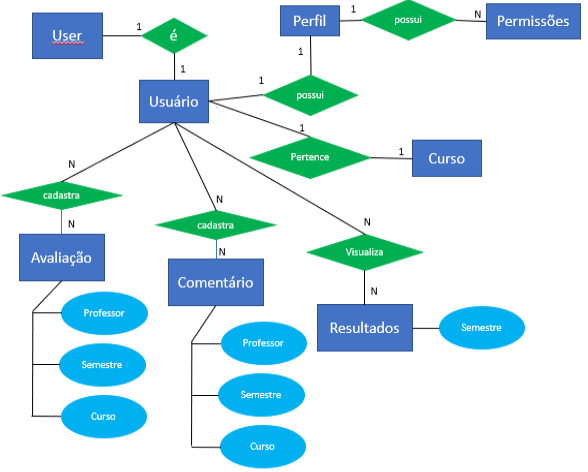
\includegraphics{modelo_conceitual.png}
\caption{Modelo Conceitual}
\label{fig:modelo_conceitual}
\end{figure}
 
A entidade User possui um relacionamento direto com a  entidade Usuário, o que nos diz que um User é um Usuário. O Usuário por sua vez possui um Perfil que tem uma ou mais Permissões. Ele também pode cadastrar uma ou mais Avaliações, um ou mais Comentários e visualizar um ou mais Resultados. Um Usuário também pertence a um Curso

\section{Autenticação}
\label{section:autenticacao}
Inicialmente para atender a demanda no processo de identificação que existe em qualquer sistema web, foi pensado em um \textit{login} básico para autenticação, possuindo apenas usuário e senha. Entende-se como login o processo para acessar um sistema informático restrito, utilizando credenciais que são previamente cadastradas pelo usuário nesse sistema, com a finalidade da identificação do utilizador. Contudo, como os objetivos da solução apresentados no capítulo \ref{chap:introducao} possuem um contexto sensível, o login, dessa forma mais simples abrangeria qualquer usuário logado na internet que possuísse o caminho do sistema, não sendo interessante, pois os mesmos teriam acesso a resultados que possuem informações direcionadas apenas a comunidade acadêmica da UFBA.
Para delimitar o acesso ao \ac{SICAD}, foi utilizado o módulo de autenticação\footnote{Autenticação UFBA. Disponível em <\url{www.autenticacao.ufba.br}>.} disponibilizado pela universidade. Seu emprego segue o seguinte processo: uma aplicação no ato do login faz uma requisição ao sistema de autenticação, que por sua vez valida esta mesma requisição e, se positiva, retorna o \textit{username} \footnote{Username é uma palavra inglesa com tradução livre para “nome de usuário”. É a identificação do usuário para acessar uma rede de computadores ou um determinado serviço na internet.} do usuário cadastrado na rede da universidade. Na Figura \ref{fig:processo_autenticacao} é demonstrado o fluxograma do processo.

\begin{figure}
\centering
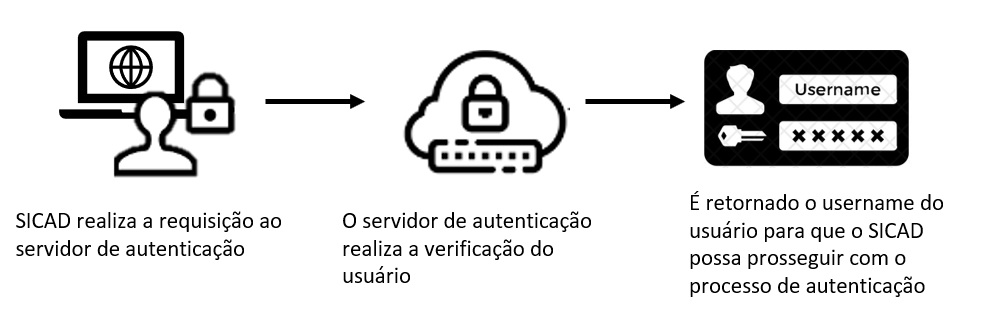
\includegraphics[scale=0.50]{processo_autenticacao.jpg}
\caption{Fluxograma da Requisição de Autenticação}
\label{fig:processo_autenticacao}
\end{figure}

Dessa forma, o acesso à aplicação fica restrito a quem possui cadastro na universidade, não expondo assim quaisquer informações à usuários que não são elegíveis para utilizar o sistema.

\section{Usuário e Segurança}
\label{subsec:userseg}
No processo de desenvolvimento da autenticação ficou clara a necessidade da implementação de uma camada de segurança, visto que a resposta à requisição feita juntamente a \ac{UFBA} retorna a identificação do usuário, ou seja, o username sem nenhum tipo proteção.

A segurança da informação é essencial no sentido de preservar o valor que a identificação do usuário representa pois ele é chave para a maioria das funcionalidades do \ac{SICAD}. Focando neste ponto, foram implementadas ações para prover segurança nos processos executados pelo sistema descritos nos passos abaixo:

\begin{itemize}
\item Como ação inicial, o usuário irá se autenticar na aplicação, consequentemente disparando uma requisição para a autenticação da \ac{UFBA};
\item São executadas todas as rotinas de validação.
Caso se obtenha uma resposta positiva, é retornado o username do usuário sem proteção para a aplicação que solicitou a requisição;
\item O \ac{SICAD}, antes de persistir a informação no banco de dados, utiliza a função de hash SHA256 com salt, que será abordada com mais profundidade no subtópico \ref{sec:seguranca}, para criptografar o username utilizado como informação chave na utilização do sistema. Para melhor fixação, o fluxo do processo está representado na figura \ref{fig:fluxograma_criptografia}.
\end{itemize}

\begin{figure}
\centering
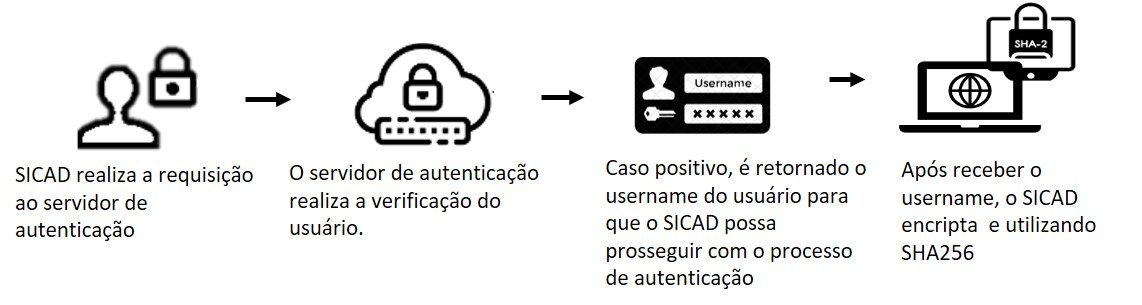
\includegraphics[scale=0.80]{fluxograma_criptografia.jpg}
\caption{Fluxograma das Etapas do Processo de Criptografia do Username.}
\label{fig:fluxograma_criptografia}
\end{figure}

Por conseguinte, com o usuário criptografado e devidamente protegido a navegação na aplicação se faz de forma segura.

\section{Perfis}
\label{section:perfil}
A utilização de perfis de usuários está atrelada à restrição de acesso à certas funcionalidades do sistema, que, embora não elimine todos os riscos à segurança da informação, diminui incidentes que possam ocorrer.

No \ac{SICAD} foi implementado o controle de perfis considerando critérios de segurança de confidencialidade e integridade  para que não ocorra a quebra dos mesmos gerando venerabilidades.

\section{O controle de acesso}
Um processo de segurança essencial assegurado pelos critérios de segurança é o controle de acesso. É difícil imaginar como qualquer sistema teria condições minímas de continuar funcionando sem ele e por isso é imprescindível sua implementação.

\subsection{Controle  de  Acesso  Baseado  em  Papéis}
Considerando o cenário dos acessos que foram pensados para o \ac{SICAD}, foi escolhido o modelo de \textit{controle  de  acesso  baseado  em  papéis} devido a sua adequação à aplicação.

Para \citep{sandhu1997}, o modelo Role Based Access Control \ac{RBAC} flexibiliza o gerenciamento do controle de acesso através da adição de um componente que intermedeia usuários e permissões. Este considera quatro componentes básicos:
\begin{itemize}
\item \textbf{Usuários}: Podem ser seres humanos ou outros agentes autônomos, tais como robôs, agentes de software e computadores;
\item \textbf{Permissões}: São os direitos de executar uma ou mais ações ou operações sobre objetos do sistema;
\item \textbf{Papéis}: São os intermediários entre os usuários e as permissões. Em vez de conceder permissões diretamente aos usuários, as permissões são concedidas aos papéis. Papéis são funções distintas dentro do sistema, como por exemplo Administrador, Moderador e etc. Usuários são associados a um ou mais papéis.  
\item \textbf{Sessões}: Quando um usuário acessa o sistema, ele inicia uma \textbf{sessão}; durante  essa  sessão, pode haver  um  ou  mais  papéis ativos. Conforme a especificação do modelo, o usuário pode ter ou não o poder de decidir quais papéis ativar em um dado momento.
\end{itemize}

Partindo desses quatro componentes foram criados os papéis e permissões do sistema que poderão ser visualizados através da tabela \ref{tab:papelperm}.

% ######## init table ########
\begin{table}
 \centering
% distancia entre a linha e o texto
 {\renewcommand\arraystretch{1.25}
 \begin{tabular}{ l l }
  \cline{1-1}\cline{2-2}  
    \multicolumn{1}{|p{4cm}|}{\textbf{Papel} \centering } &
    \multicolumn{1}{p{6cm}|}{\textbf{Permissão} \centering }
  \\  
  \cline{1-1}\cline{2-2}  
    \multicolumn{1}{|p{4cm}|}{Administrador} &
    \multicolumn{1}{p{6cm}|}{incluir, alterar, visualizar, bloquear, desbloquear, denunciar em todos os módulos do sistema considerando autoria de todos os papéis}
  \\  
  \cline{1-1}\cline{2-2}  
    \multicolumn{1}{|p{4cm}|}{Utilizador} &
    \multicolumn{1}{p{6cm}|}{incluir, alterar, ocultar, mostrar, denunciar nos módulos de comentários e avaliação considerando autoria individual do papel}
    \\
      \cline{1-1}\cline{2-2}  
        \multicolumn{1}{|p{4cm}|}{Moderador} &
        \multicolumn{1}{p{6cm}|}{visualizar, bloquear, desbloquear em todos os módulos do sistema considerando autoria de todos os papéis}
  \\
  \hline
 \end{tabular} }
 \caption{Papéis e Permissões}
  \label{tab:papelperm}
\end{table}

Um usuário poderá ter o papel de administrador ou utilizador associado. Como padrão quando o mesmo realiza o login já é atribuído a ele o papel de \textit{utilizador}.

Além dos papéis e permissões citados acima, o \ac{SICAD} conta com módulos, que são partes do sistema responsáveis por uma ou mais tarefas definidas, que estão por sua vez associados aos papéis como é demonstrado pela Tabela \ref{tab:papelmod} e especificados com mais detalhes no capítulo \ref{sec:principaisfuncionalidades}.

% ######## init table ########
\begin{table}
 \centering
% distancia entre a linha e o texto
 {\renewcommand\arraystretch{1.25}
 
 \begin{tabular}{ l l }
  \cline{1-1}\cline{2-2}  
    \multicolumn{1}{|p{3.850cm}|}{\textbf{Módulo} \centering } &
    \multicolumn{1}{p{7.217cm}|}{\textbf{Papel} \centering }
  \\  
  \cline{1-1}\cline{2-2}  
    \multicolumn{1}{|p{3.850cm}|}{Comentário} &
    \multicolumn{1}{p{6.217cm}|}{Administrador, Utilizador}
  \\  
  \cline{1-1}\cline{2-2}  
    \multicolumn{1}{|p{3.850cm}|}{Avaliação} &
    \multicolumn{1}{p{6.217cm}|}{Administrador, Utilizador}
  \\  
    \cline{1-1}\cline{2-2}  
    \multicolumn{1}{|p{3.850cm}|}{Resultados} &
    \multicolumn{1}{p{6.217cm}|}{Administrador, Utilizador}
  \\  
    \cline{1-1}\cline{2-2}  
    \multicolumn{1}{|p{3.850cm}|}{Ajuda} &
    \multicolumn{1}{p{6.217cm}|}{Administrador, Utilizador}
  \\  
    \cline{1-1}\cline{2-2}  
    \multicolumn{1}{|p{3.850cm}|}{Carga} &
    \multicolumn{1}{p{6.217cm}|}{Administrador}
  \\  
    \cline{1-1}\cline{2-2}  
    \multicolumn{1}{|p{3.850cm}|}{Moderação} &
    \multicolumn{1}{p{6.217cm}|}{Administrador}
  \\  
    \cline{1-1}\cline{2-2}  
    \multicolumn{1}{|p{3.850cm}|}{Configurações} &
    \multicolumn{1}{p{6.217cm}|}{Administrador}
  \\  
  \hline
 \end{tabular}}
 \caption{Papéis e Módulos}
 \label{tab:papelmod}
\end{table}
O modelo \ac{RBAC}, nos permite  definir permissões e impor restrições aos papéis que utilizam os módulos de acordo com a necessidade da aplicação, resultando em mais proteção e boa gestão da informação oferecida pelo sistema.


\section{Anonimato}
\label{sec:anonimato}

Segundo o dicionário Houaiss, anonimato significa ``1. Que não tem o nome ou a assinatura do criador; 2. Que ou aquele que não revela seu nome'' \cite[p. 7]{houasis2001}. Podemos perceber que em diversas situações cotidianas e principalmente em publicações na internet este conceito é bastante utilizado: a manifestação do pensamento não identificado.

Na avaliações praticadas pela universidade, existe um momento em que o discente pode expressar sua opinião sobre o desempenho do docente em sala de aula de acordo com a disciplina avaliada. Todo processo é realizado de forma não identificada e o professor não possui acesso acerca quem realizou a avaliação. O conceito de anonimato se perde uma vez que para realizar qualquer operação o discente tenha que realizar um login, logo a partir desse ponto utilizaremos a não identificação para referir-se-á qualquer situação que arremeta ao conceito de anonimato.

A fim de realizar um estudo sobre o alcance e utilização da aplicação, assim como a definição de um ponto crucial que seria a implementação da avaliação nos mesmo moldes do \ac{SIAV}, levando em consideração a identificação do aluno, um questionário foi aplicado para obtenção de dados base acerca desse tópico. 
Foi utilizado para coleta de informação o procedimento do tipo pesquisa de levantamento. O modelo escolhido foi do tipo questionário, o qual foi desenvolvido utilizando a ferramenta do Google Forms, pois foi a mais simples de chegar no público alvo desejado. O questionário completo aplicado encontra-se descrito no apêndice \ref{ape:apendice}.

Consideremos as perguntas aplicadas \textit{"Se existisse uma aplicação onde fosse possível a inclusão de comentários sobre determinada disciplina dada por um professor em um determinado semestre, você utilizaria essa aplicação?"} como \textbf{Pergunta A} e \textit{ 
"Se você fosse realizar um determinado comentário sobre uma disciplina nessa aplicação, você gostaria de se identificar?"} como \textbf{Pergunta B}, onde temos \textbf{sim} e \textbf{não} como alternativas de resposta e se o resultado do primeiro  questionamento for positivo estará relacionado com a possibilidade de resposta do segundo questionamento. O questionário foi aplicado entre agosto e setembro do ano de 2019 em um grupo destinado à comunidade da universidade, criado na rede social Facebook\footnote{Facebook. Disponível em <\url{www.facebook.com/}>. Acesso em: 20 nov. 2019} chamado \textit{UFBA}, e foram obtidas setenta e duas respostas. 

\begin{figure}
\centering
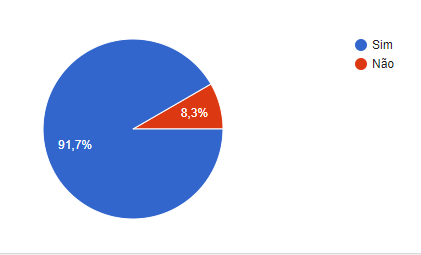
\includegraphics[scale=0.8]{pergunta_a.png}
\caption{Pergunta A}
\label{fig:pergunta_a}
\end{figure}

\begin{figure}
\centering
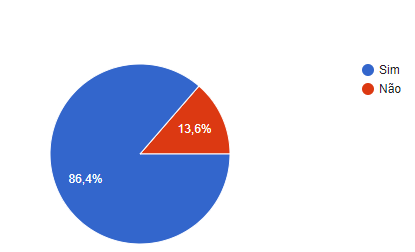
\includegraphics[scale=0.8]{pergunta_b}
\caption{Pergunta B}
\label{fig:pergunta_b}
\end{figure}

Pelos resultados do questionário, visualizados nas Figuras \ref{fig:pergunta_a} e \ref{fig:pergunta_b}, fica claro que os 91,7\% da população de estudantes estudada utilizaria o SICAD e que 86,4\% gostariam de fazê-lo de forma não identificada. Esses dados foram levados em consideração no desenvolvimento deste trabalho e o sistema hoje realiza as avaliações e comentários não identificando seus autores.


\section{ Principais Funcionalidades}
\label{sec:principaisfuncionalidades}

Como descrito no inicio do Capítulo \ref{chap:solucaoproposta}, esta solução foi pensada como uma união da funcionalidade de avaliar os docentes da UFBA com uma nova funcionalidade de realizar comentários.

Os \textit{comentários} são uma forma de o discente compartilhar sua experiência vivida na sala de aula e que poderá ser visualizada por todos os usuários que são elegíveis para utilizar o sistema.

As \textit{avaliações} são um parecer que um discente fornece referente a um docente e seu trabalho ministrando uma dada disciplina, em um dado semestre. O conceito de avaliação foi baseado no que já é utilizado pela universidade e nos trabalhos relacionados estudados.

Contabilizando as avaliações realizadas pelos estudantes, o \ac{SICAD} oferece \textit{resultados}, apresentando de forma simples e transparente a contabilização dos itens avaliados.

O utilizador do sistema dispõe também do recurso de \textit{ajuda}, através do qual poderá tirar possíveis dúvidas a respeito do que são comentários, avaliações e resultados a qualquer momento. Podemos observar na figura \ref{fig:home_administrador} a tela inicial do sistema.
\begin{figure}
\centering
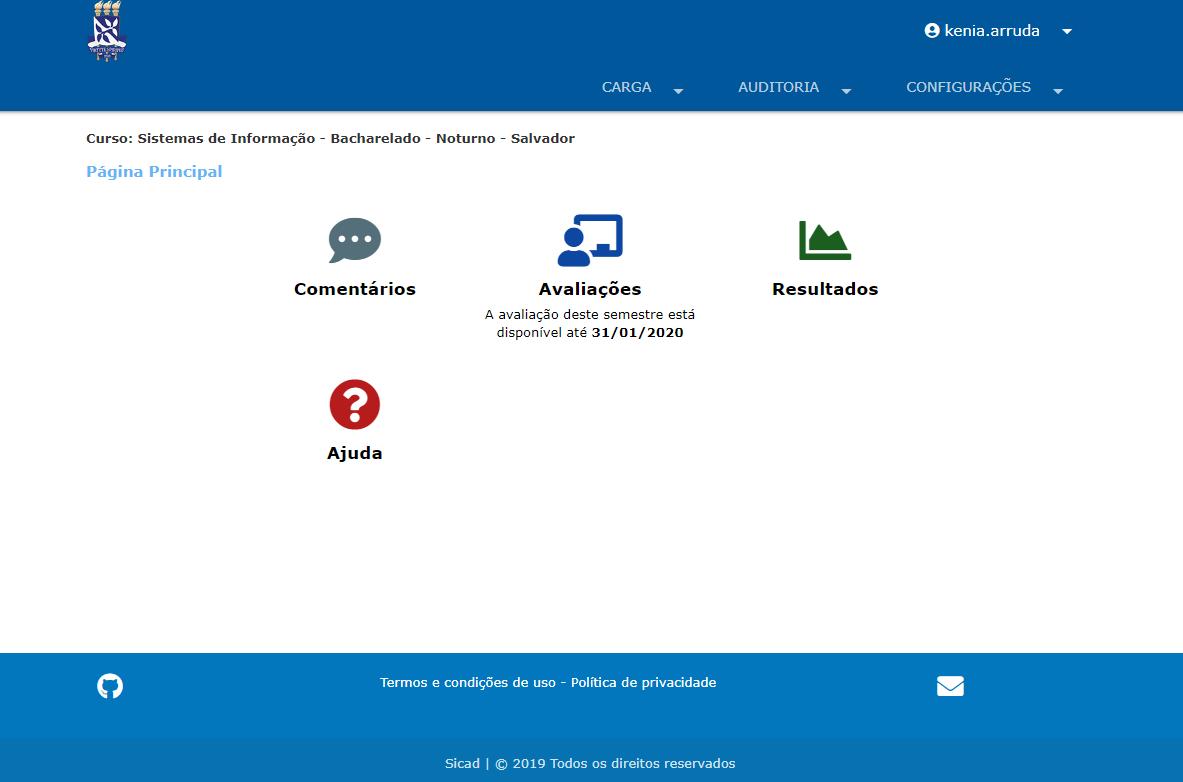
\includegraphics[scale=0.5]{home_administrador2.png}
\caption{Tela Inicial do SICAD.}
\label{fig:home_administrador}
\end{figure}

Nos próximos tópicos serão descritas as principais funcionalidades de cada módulo disponível no \ac{SICAD}.

\subsection{Comentário}
\label{subsec:comentario}
Um comentário tem por objetivo o compartilhamento das experiências vividas e informações pertinentes de uma determinada combinação de disciplina, professor e semestre cursado. Espera-se que sejam compartilhadas informações que gerem conhecimento base para os que não conhecem a disciplina e/ou o trabalho do professor naquela disciplina.

Além dos objetivos citados, os comentários também poderão ser utilizados como sugestões, elogios e críticas sobre o conhecimento ministrado na combinação disciplina-professor-semestre avaliada. Eles deverão seguir a convenção de não possuir palavras de baixo de calão, vulgo palavrões, evitando assim constrangimento e ofensas. A Tabela~\ref{tab:comentario} apresenta um exemplo de comentário.

\begin{table}[h]
 \centering
 {\renewcommand\arraystretch{1.25}
 \begin{tabular}{ l l }
  \cline{1-1}\cline{2-2}  
    \multicolumn{1}{|p{7.850cm}|}{\par \textbf{Disciplina:} Álgebra Linear
    \par \textbf{Professor:} Fulano de Tal
    \par \textbf{Comentário:} Esse professor é muito atencioso! Aprendi a disciplina rapidamente. Acho que ele passa muito trabalho extra classe.}
  \\  
  \hline
 \end{tabular}}
 \caption{Exemplo de Comentário}
 \label{tab:comentario}
\end{table}

Para que validação da convenção dos comentário seja realizada no momento do seu cadastro foi desenvolvido um algoritmo que compara os radicais da palavras utilizadas em sua escrita utilizando a stemmização com um banco de dados previamente cadastro com os radicais de palavrões conhecidos. 

O módulo de comentário possui as seguintes ações:

\begin{itemize}
\item \textbf{Incluir}: Esta funcionalidade permite o usuário incluir um comentário que ficará disponível para os demais usuários. Uma vez realizado, o mesmo passa a possuir a situação de \textit{comentário público}. É obrigatório o utilizador informar a disciplina, o semestre, o professor e o comentário a ser realizado. Na Figura \ref{fig:incluir_comentario} observamos um exemplo a tela de inclusão.

\begin{figure}
\centering
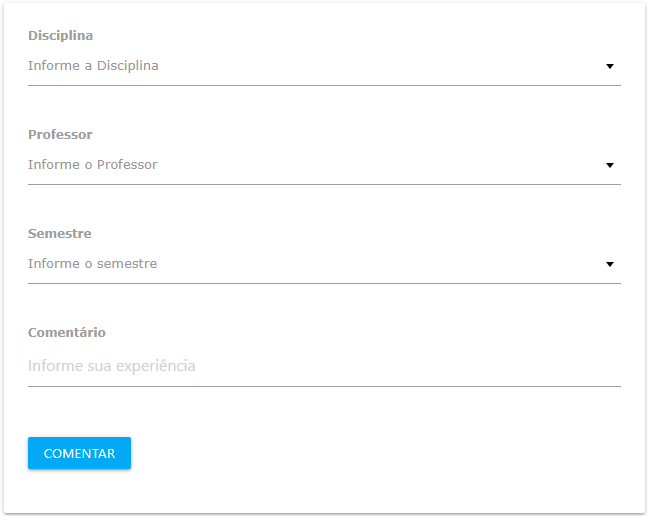
\includegraphics[scale=0.59]{incluir_comentario2.png}
\caption{Tela de Inclusão de Comentário.}
\label{fig:incluir_comentario}
\end{figure}

\item \textbf{Visualizar}: Esta funcionalidade permite ao usuário consultar tanto os seus próprios comentários realizados como os que foram incluídos por outros usuários. Podemos visualizar nas Figuras \ref{fig:comentarios} e \ref{fig:visualizacao_meu_comentario} respectivamente.

\begin{figure}
\centering
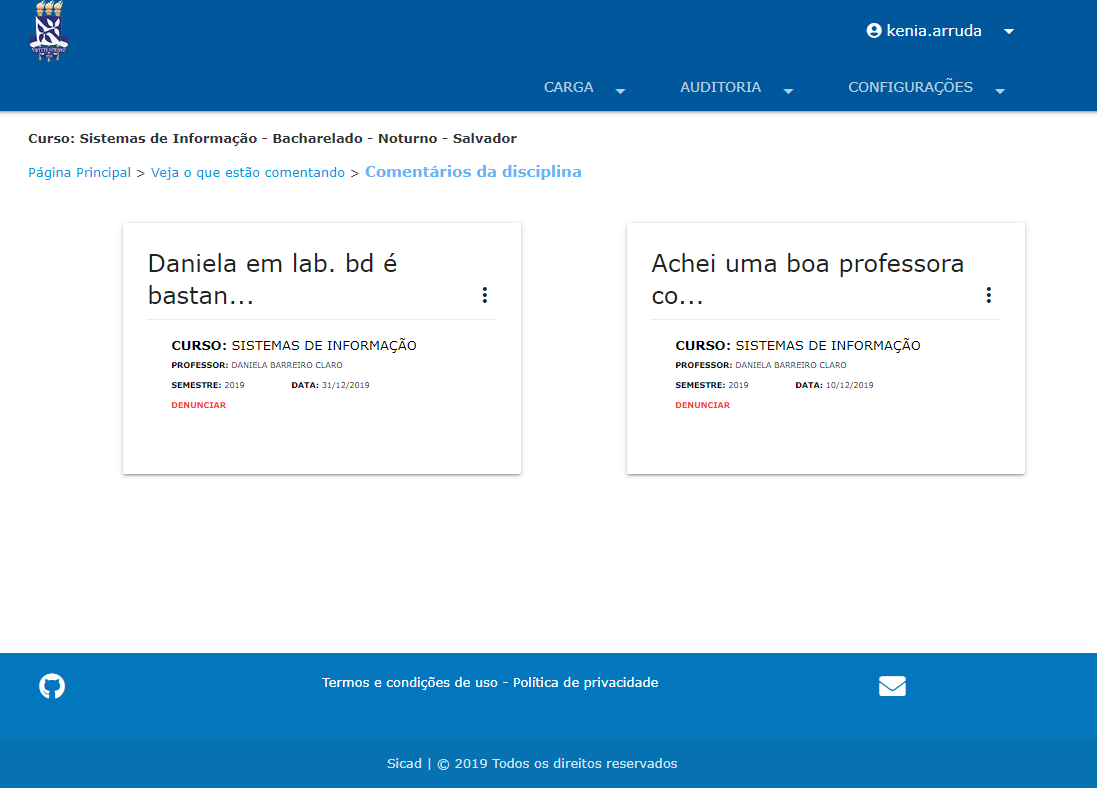
\includegraphics[scale=0.5]{comentarios2.png}
\caption{Tela de Visualização de Todos os Comentários.}
\label{fig:comentarios}
\end{figure}

\begin{figure}
\centering
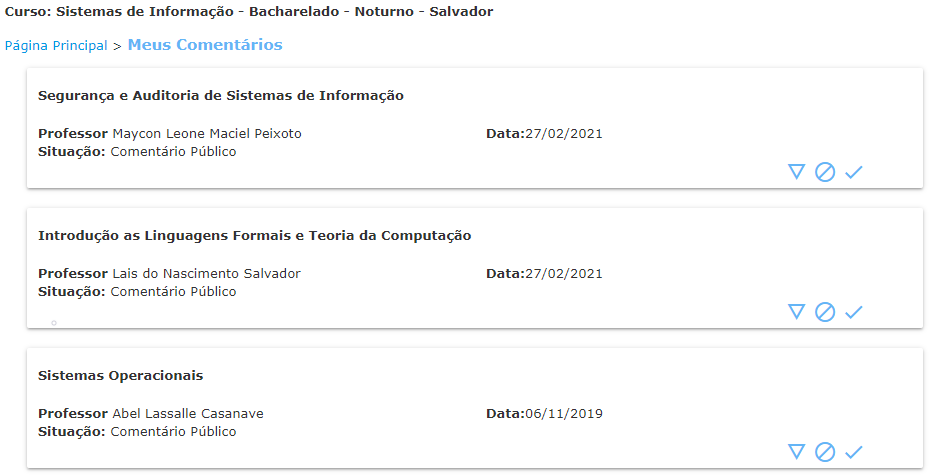
\includegraphics[scale=0.7]{visualizacao_meu_comentario.png}
\caption{Tela de Visualização dos Comentários Realizados pelo Usuário.}
\label{fig:visualizacao_meu_comentario}
\end{figure}

\item \textbf{Ocultar/Mostrar}: Essas funcionalidades permitem ao usuário ocultar um comentário realizado, ou seja, esse comentário não poderá ser mais visualizado pelos demais, passando a ter a situação de \textit{comentário oculto}, podendo apenas ser consultado pelo próprio utilizador. Para revogar o privilégio de ocultamento o mesmo poderá utilizar a função de mostrar, tornando o \textit{comentário publico} novamente. Nas Figuras \ref{fig:comentario_oculto} e \ref{fig:comentario_publico} visualizamos exemplos.

\item \textbf{Denunciar}: Um comentário poderá ser denunciado quando o mesmo infringir a convenção, ou seja, ter palavras de baixo calão em seu conteúdo. Comentários escritos de forma pejorativa dissonante dos objetivos propostos deverão ser denunciados. Todos os participantes que utilizam \ac{SICAD} poderão denunciar comentários inapropriados. A contabilização das denúncias é realizada pelo sistema e o administrador que realiza a moderação pode bloquear esses comentários denunciados e os mesmos não ficarão mais disponíveis para visualização de todos nas aplicação.

\begin{figure}
\centering
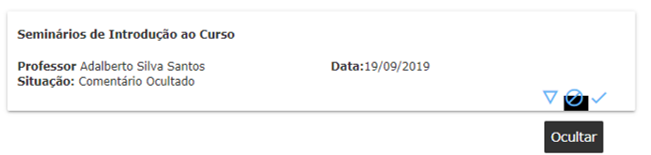
\includegraphics[scale=0.7]{comentario_oculto.png}
\caption{Imagem de um Comentários Oculto.}
\label{fig:comentario_oculto}
\end{figure}

\begin{figure}
\centering
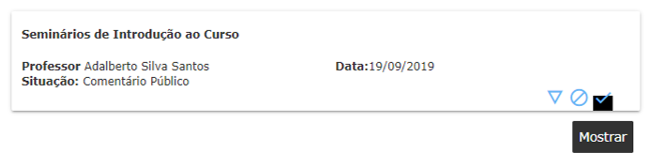
\includegraphics[scale=0.7]{comentario_publico.png}
\caption{Imagem de um Comentários Público.}
\label{fig:comentario_publico}
\end{figure}



\end{itemize}
\subsection{Avaliação}

Uma avaliação é uma análise que um discente fornece referente a um docente e/ou seu trabalho ministrando uma dada disciplina em um dado semestre. Ela é composta de avaliações sobre a didática, relacionamento com os alunos e domínio de conteúdo, uma escala de recomendação e atribuições de palavras-chaves (\textit{tags}). A avaliação é uma combinação professor, disciplina e semestre, que são itens geralmente levados em consideração para uma decisão da matrícula de um aluno.

O módulo de avaliação possui as seguintes ações:
\begin{itemize}
\item \textbf{Incluir}: Esta funcionalidade permite ao usuário incluir uma avaliação docente onde serão avaliados os critérios de didática, relacionamento com os alunos e domínio de conteúdo, baseados nos mesmos conceitos utilizados pelo SIAV, onde será atribuído um gostei ou não gostei à cada item.

O usuário pode associar palavras-chaves (em inglês, tags), explicadas com mais detalhe no subtópico \ref{subsection:configuracao}, na inclusão da avaliação. Ao final, o mesmo deverá informar na escala de 1 a 5 estrelas qual o nível de recomendação do docente lecionando a disciplina avaliada. Por padrão a recomendação está apontada para o 3. 

Fica obrigatório o utilizador informar a disciplina, o semestre e o professor. Na Figura \ref{fig:incluir_avaliacao}  podemos visualizar a tela de inclusão de uma avaliação docente.

\begin{figure}
\centering
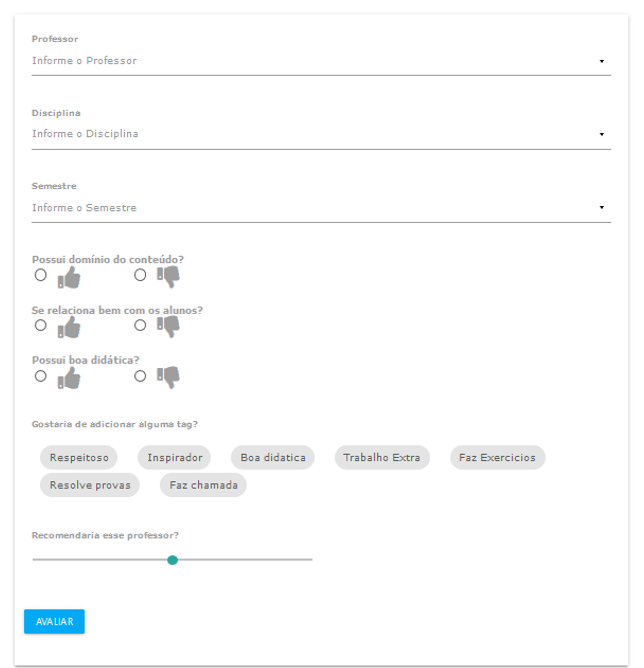
\includegraphics[scale=0.5]{incluir_avaliacao.png}
\caption{Incluindo uma Avaliação Docente.}
\label{fig:incluir_avaliacao}
\end{figure}

\item \textbf{Visualização}: Esta funcionalidade permite o usuário visualizar suas avaliações realizadas. Na Figura \ref{fig:visualizacao_minha_avaliacao} observamos as avaliações do utilizador.

\begin{figure}
\centering
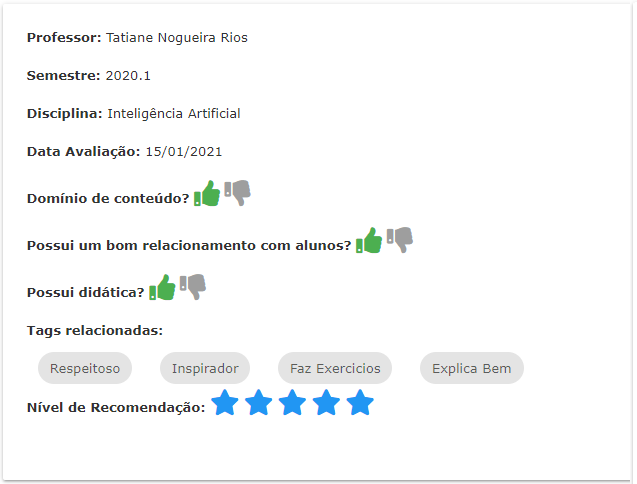
\includegraphics[scale=0.7]{visualizacao_minha_avaliacao.png}
\caption{Visualização das Avaliações do Usuário.}
\label{fig:visualizacao_minha_avaliacao}
\end{figure}

\end{itemize}
\subsection{Resultados}
Um resultado tem como objetivo demonstrar de forma sintética as avaliações realizadas ao longo do semestre, auxiliando assim o discente na escolha das disciplinas que irão compor sua  grade.

Os resultados são apresentados por semestre e dentro do mesmo serão visualizados os resumos por professor. Na Figura \ref{fig:resultados} observamos um exemplo de resultado.

\begin{figure}
\centering
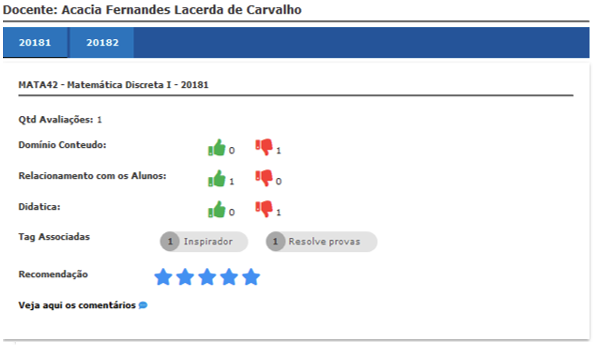
\includegraphics[scale=0.7]{resultados.png}
\caption{Demostração dos Resultados.}
\label{fig:resultados}
\end{figure}

Como é visualizado na imagem \ref{fig:resultados}, uma contagem do conceito de "gostei" e "não gostei" dos itens domínio de conteúdo, relacionamento com o aluno e didática é apurada. É realizada também a contagem da quantidade que uma palavra-chave foi associada na avaliação. Já para a recomendação, na sua contabilização é utilizada a média aritmética simples dada pela formulação matemática:

\begin{equation}
\bar{x}=\frac{\sum{x_{i}}}{n} 
\end{equation}

onde xi são as recomendações(atribuídas em estrela) e n a quantidade das recomendações.

Através dos resultados, os discentes poderão visualizar os comentários de acordo com a disciplina, o semestre e o professor selecionado.

\subsection{Ajuda}
\label{subsection:ajuda}
Pensando na experiência do utilizador e para proporcionar uma ferramenta de respostas à questionamentos frequentes foi desenvolvido um módulo de ajuda para os utilizadores do SICAD. Nele é possível tirar dúvidas acerca do que são comentários, avaliação e resultados. Podemos visualizar na figura \ref{fig:ajuda} o módulo de ajuda.

\begin{figure}
\centering
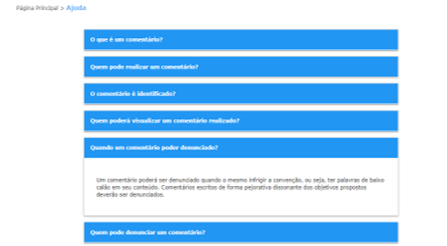
\includegraphics[scale=0.6]{ajuda.png}
\caption{Demonstração da Ajuda.}
\label{fig:ajuda}
\end{figure}

\subsection{Carga}
\label{subsection:carga}
As informações sobre os cursos, disciplinas e professores que são utilizados pelo SICAD são disponibilizadas para o público no site da Superintendência de Administração Acadêmica (SUPAC) \footnote{SUPAC. Disponível em <\url{https:www.supac.ufba.br}>. Acesso em: 13 nov. 2019} na forma de um documento HTML\footnote{HTML. É  uma linguagem de marcação utilizada na construção de páginas na Web.}.

O processo de desenvolvimento do web scraping que foi empregado nesta solução foi baseado no trabalho realizado por \citeauthor{assis2017meuhorario} no projeto do MeuHorário2\footnote{MeuHorário2. Disponível em <\url{www.meuhorarioufba.com.br/}>. Acesso em: 13 nov. 2019}. Inicialmente foram definidas três etapas, utilizando o tipo informação que passa a ser o foco da extração: cursos, disciplinas e professores.  Em cada etapa, foi desenvolvida uma \textit{task}, conceito utilizado pela linguagem de programação Ruby, que são tarefas, ou seja, instruções a serem executadas mesmo que a aplicação não esteja em execução. 

A primeira tarefa desenvolvida foi a extração de cursos, através de uma página de listagem dos cursos da UFBA. Foram extraídos os dados: nome e código do curso. Podemos visualizar na Figura \ref{fig:lista_cursos} como a informação é apresentada pela página da UFBA.

\begin{figure}
\centering
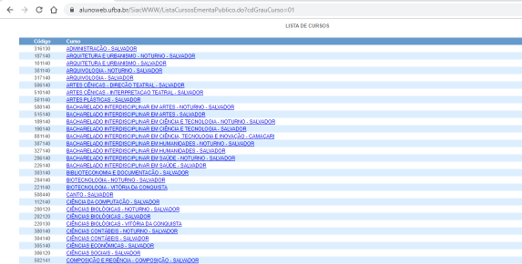
\includegraphics[scale=0.9]{lista_cursos.png}
\caption{Lista de Cursos.}
\label{fig:lista_cursos}
\end{figure}

A segunda tarefa desenvolvida foi a extração das disciplinas de cada curso. No site da \ac{SUPAC} existe uma área que possui links para os guias de matrícula de cada curso. Os cursos são divididos por áreas e a partir dos guias, é possível obter informações sobre as disciplinas sendo assim habilitada uma associação entre curso e disciplina. Na figura \ref{fig:disciplinas} podemos visualizar um exemplo da listagem das disciplinas de um curso no site da SUPAC.

\begin{figure}[ht!]
\centering
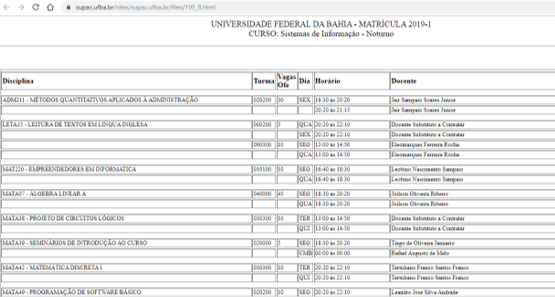
\includegraphics[scale=0.8]{disciplinas.png}
\caption{Lista de Disciplinas de um Curso.}
\label{fig:disciplinas}
\end{figure}

Finalizando o conjunto das tarefas, a extração da relação dos professores também se dá pelo guia de matrícula, visto que a partir dele é possível obter a informação dos professores como é representado na Figura \ref{fig:disciplinas} . 

\subsection{Moderação}
\label{subsec:moderacao}
Para \citep{netosolanca2007}, a auditoria é uma atividade que reúne a análise das operações, processos, sistemas e responsabilidades gerenciais de uma determinada entidade, com o intuito de validar sua conformidade com certos objetivos e políticas institucionais, regras, orçamentos, normas ou padrões.

Partindo do conceito de auditoria, uma das suas vertentes seria a moderação de conteúdo. Este por sua vez se encaixa no contexto do SICAD, pois os comentários realizados, embora devam seguir do padrão de não possuir palavras de baixo calão, os palavrões, podem se tornar ofensivos, havendo a necessidade de uma intervenção do moderador.
De acordo com \cite{SMITH2019} existem quatro tipos de moderação:
\begin{itemize}
\item \textbf {Pré-moderação: }Com a pré-moderação, você emprega moderadores para verificar novamente o conteúdo enviado pelo seu público-alvo antes que ele fique visível ao público; 
\item \textbf {Pós-moderação: }Ao contrário da pré-moderação, a pós-moderação abre caminho para conversas em tempo real e postagem imediata, porque o conteúdo é verificado depois de publicado;
\item \textbf {Moderação distribuída: }Um sistema de classificação é usado com moderação distribuída, permitindo que os membros da comunidade votem em determinados envios. Um exemplo de moderação distribuída é o site Stack Overflow,\footnote{Stack Overflow Disponível em: <url:{www.pt.stackoverflow.com}/>} onde os usuários votam nas respostas mais adequadas para uma pergunta realizada;
\item \textbf {Moderação automatizada: } A moderação automatizada funciona usando aplicativos específicos de moderação de conteúdo para filtrar certas palavras ofensivas e conteúdo multimídia. A detecção de postagens inapropriadas se torna automática e mais integrada. 
\end{itemize}

O SICAD utiliza dois dos tipos de moderação citados, que são os de pós moderação e moderação automatizada. Devido ao seu conteúdo sensível, os comentários são moderados quando necessário. Como dado pessoal sensível, a lei Nº 13.709, de 14 de agosto de 2018 artigo 5º nos diz ``Dado pessoal sensível é informação relativa a origem racial ou étnica, convicção religiosa, opinião política, filiação a sindicato ou organização, saúde, vida sexual ou dado genético ou biométrico''.  Contudo, o artigo 5º nos fornece um conceito de dado sensível muito engessado e entendendo que a informação armazenada referente aos comentários que são registrados no sistema pode de algum jeito gerar constrangimento se exposta, foi desenvolvido um módulo de moderação dos comentários realizados pelos usuários.

A moderação neste momento inicial será realizada por um usuário com papel Moderador associado a ele. Observa-se a pós-moderação, quando o moderador pode visualizar todos os comentários realizados, e os que forem denunciados ou tiver seu conteúdo escrito de forma pejorativa, poderão ser bloqueados. Quando está nesta situação, o comentário automaticamente não ficará mais disponível para consulta dos demais. Também é papel do Moderador manter atualizada a lista de palavras restritivas utilizada pela rotina de inserção de comentários. 

A moderação automatizada foi implementada pensando em não permitir que o usuário realize um comentário pejorativo, auxiliando o moderador e mantendo um feed \footnote{O feed é um fluxo de conteúdo que permite rolagem. O conteúdo é exibido em blocos de aparência semelhante que se repetem um após o outro.}saudável com elogios e críticas construtivas. Utilizando a técnica de stemmização, quando o usuário escreve um comentário que possui alguma palavra que está contida numa lista de palavras restritivas previamente preenchida, o comentário não é persistido no banco de dados.  

Através dos pontos citado acima entendemos a importância da utilização da moderação para manutenibilidade dos comentários dentro do conceito da proposta.

\subsection{Configuração}
\label{subsection:configuracao}
O módulo de configuração foi implementado para suprir as informações críticas necessárias para o funcionamento da aplicação. Nele o Administrador pode cadastrar e dar manutenção nas palavras-chave utilizadas pela avaliação, nas palavras restritivas utilizadas no módulo de comentários e informar o período em que a avaliação ficará disponível para utilização dos usuários.

São consideradas as tags default \footnote{Default é um termo técnico utilizado em computação e pode ser utilizado tanto para referir-se a um valor pré-definido, que o sistema computacional assume.} do sistema as opções "Respeitoso", "Inspirador", "Trabalho Extra", "Faz Exercícios", "Resolve provas", "Faz chamada", "Faz substitutiva", "Explica Bem", "Comprometido", "Comunicativo"e "Bom material didático" cadastradas pelo Administrador. Elas foram pensadas na tentativa de englobar competências docentes avaliadas pelo SIAV de uma forma mais interativa para o usuário mesclando com tags ja utilizadas por outros sistema estudo os trabalhos relacionados.

Para as palavras de baixo calão foram pesquisadas palavras consideradas como xingamento dentro da língua brasileira e cadastradas pelo Administrador nas forma de seus radicais respeitando a stemmização.

\chapter{Avaliação}
\label{chapter:avaliacao}

Um sistema informático pode apresentar problemas, seja ele em um sua interface como na sua usabilidade, e isso pode gerar como consequência frustração por parte do utilizador a ponto de o mesmo não voltar mais a utilizá-lo.
É por isso que uma avaliação se faz necessária, na qual um  avaliador faz um julgamento sobre a qualidade de uso da solução e identifica problemas na interação e na interface, sendo assim possível corrigir os problemas relacionados à usabilidade antes de introduzir o sistema no dia-a-dia dos usuários.

\section{Objetivo da avaliação }
Para garantir que uma avaliação obtenha sucesso é de extrema importância definir quais são os objetivos da avaliação. Esses objetivos determinam quais aspectos relacionados ao uso do sistema devem ser investigados. Neste trabalho vamos considerar os seguintes objetivos:
\begin{itemize}
 
 \item{\textbf{Avaliar o objetivo e satisfação dos módulos de comentários e avaliação junto ao usuário:}} Deve-se avaliar a usabilidade da interface; o quão fácil foi aprender a usar a interface.
 \item{\textbf{Identificar problemas específicos:}} Identificar aspectos da interface, que quando usados no contexto alvo, causam resultados inesperados ou confusão entre os usuários.
\end{itemize}

\section{Forma de avaliação}

Segundo \cite{polson1992cognitive}, usabilidade é um termo usado para definir a facilidade com que as pessoas podem empregar uma ferramenta ou objeto a fim de realizar uma tarefa específica e importante. 

A fim de aplicar o conceito de usabilidade apresentado, foi considerada na fase de levantamento da informações uma amostra de trinta (30) usuários utilizando a técnica de \textit{Amostragem por Escolha}\footnote{ Na amostragem por escolha o pesquisador busca na população uma parte dela que interessa, ou seja, os participantes são escolhidos por terem uma ou mais características específicas.} e aplicado um formulário do tipo questionário, utilizando a ferramenta do Google Forms, onde se pede para responder se o objetivo das funcionalidades realizar comentário e avaliação foram alcançados e o  grau de satisfação em relação a esses respectivos módulos, assim como foi disponibilizado um campo para responder se o usuário teve alguma dificuldade no entendimento dos módulos e um campo para sugestões de melhoria.

\section{Resultados} 
Consideremos o questionário aplicado pelo formulário de avaliação contido no apêndice deste trabalho. Da amostra selecionada somente vinte (20) pessoas responderam o questionário.
Para as perguntas 2, 4 e 5 a escala utilizada dispõe dos itens Muito Insastifeito, Insastifeito, Indiferente, Satisfeito e Muito Satisfeito, onde o termo Muito Insastifeito representa total insatisfação e o termo Muito Satisfeito representa completa satisfação.

\begin{itemize}
\item{\textbf{ Pergunta 1}}
\textit{Em relação ao módulo de comentários, o objetivo de realizar um comentário foi atingido?}.

O resultado obtido na Figura \ref{fig:grafico_pergunta1} demonstra que em todas as tentativas para a realização de um comentário no SICAD o objetivo foi atingido, ou seja, o sistema cumpre a funcionalidade descrita neste trabalho.

\begin{figure}
\centering
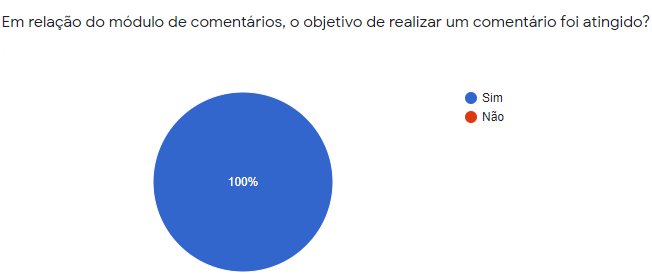
\includegraphics[scale=0.8]{grafico_pergunta1.png}
\caption{Em relação ao módulo de comentários, o objetivo de realizar um comentário foi atingido?}
\label{fig:grafico_pergunta1}
\end{figure}

\item{\textbf{ Pergunta 2}}
\textit{Como você se sente em relação ao objetivo de realizar um comentário?}.

\subitem{16 responderam que estão Satisfeitos;}
\subitem{4 responderam que estão Muitos Satisfeitos;}

Observa-se na imagem \ref{fig:grafico_pergunta2} que o grau de satisfação foi alcançado visto que o sentimento de satisfação está em evidência nas respostas.

\begin{figure}
\centering
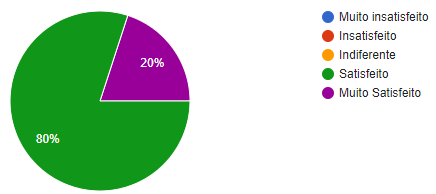
\includegraphics[scale=0.8]{grafico_pergunta2.png}
\caption{Como você se sente em relação ao objetivo de realizar um comentário?}
\label{fig:grafico_pergunta2}
\end{figure}

\item{\textbf{ Pergunta 3}}
\textit{Em relação do módulo de avaliação, o objetivo de realizar um avaliação foi atingido?}.

Como se pode observar na Figura \ref{fig:grafico_pergunta3}, em todas as tentativas na realização de uma avaliação na aplicação o objetivo foi atingido com êxito, demostrando que a funcionalidade está operando de acordo como esperado.  

\begin{figure}
\centering
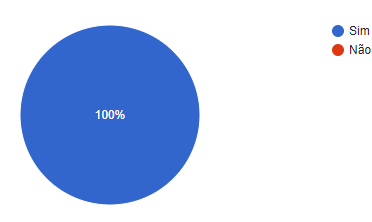
\includegraphics[scale=0.8]{grafico_pergunta3.png}
\caption{Em relação do módulo de avaliação, o objetivo de realizar um avaliação foi atingido?}
\label{fig:grafico_pergunta3}
\end{figure}

\item{\textbf{ Pergunta 4}}
\textit{Como você se sente em relação ao objetivo de realizar uma avaliação?}.

\subitem{ 12 responderam que estão Satisfeitos;}
\subitem{ 8 responderam que estão Muitos Satisfeitos;}

Segundo a Figura \ref{fig:grafico_pergunta4}, podemos visualizar que o sentimento de satisfação foi alcançado ao realizar uma avaliação.

\begin{figure}
\centering
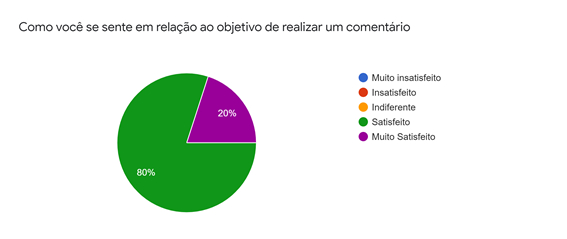
\includegraphics[scale=0.8]{grafico_pergunta4.png}
\caption{Como você se sente em relação ao objetivo de realizar uma avaliação?}
\label{fig:grafico_pergunta4}
\end{figure}

\item{\textbf{ Pergunta 5}}
\textit{Como você se sente em relação aos objetivos dos resultados apresentados pelo sistema?}.

\subitem{ 4 responderam que estão Muitos Insatisfeitos;}
\subitem{ 12 responderam que estão Satisfeitos;}
\subitem{ 4 responderam que estão Muitos Satisfeitos;}

Como podemos observar pela Figura \ref{fig:grafico_resultados}, 20\% das respostas obtidas demonstraram  sentimento de total insastifação com a forma que os resultados foram apresentados no \ac{SICAD}.Contudo, somando-se os percentuais de  sentimento de satisfação conclui-se que de 80\% da respostas se sentiram satisfeita com a forma da demostração dos resultados obtidos através da aplicação.

\begin{figure}
\centering
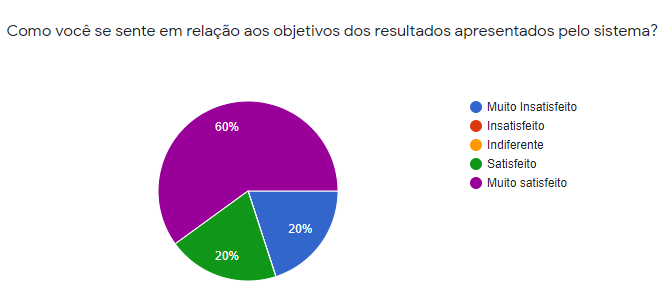
\includegraphics[scale=0.8]{grafico_resultados.png}
\caption{Como você se sente em relação aos objetivos dos resultados apresentados pelo sistema?}
\label{fig:grafico_resultados}
\end{figure}

Para finalizar o questionário aplicado, foi disponibilizado um campo para que fossem descritas, se houverem, as dificuldades encontradas na utilização da solução e possíveis sugestões para serem implementadas.

\item{\textbf{ Descreva aqui, se houverem, as dificuldades encontradas ao utilizar o sistema}}

Obteve-se as seguintes dificuldades:
\subitem{\textit{``Nos comentários achei o nome do curso de quem fez muito pequeno e data muito pequeno."}}
\subitem{\textit{``Nas minhas avaliações não informa a matéria referente à avaliação e mostrou o incorreto na didática."}}
\subitem{\textit{``O sistema não está funcional em sua forma mobile. No comentários se der pra impedir de enviar com uma notificaçãozinha e deixar editar o comentário eu acho que ficaria melhor pro usuário."}}

\item{\textbf{ Descreva aqui alguma sugestão, se houver, que queira realizar.}}


\subitem{\textit{``Disponibilizar pra cursos todos da UFBA."}}
\subitem{\textit{``Ter pra todos os cursos, um amigo meu queria usar e não pôde."}}
\subitem{\textit{"Disponibilizar mobile."}}
\subitem{\textit{``avaliação muito geral, poderia ter mais itens para avaliar"}}

\end{itemize}

Conclui-se que o objetivo da ferramenta descrita neste trabalho cumpre sua finalidade, gerando um sentimento de satisfação para registrar comentários e avaliações, assim como a visualização dos resultados obtidos, e foi possível identificar alguns pontos de melhoria que serão considerados no próximo capítulo.


\chapter{Considerações Finais}
\label{chap:consideracoes}

A falta de transparência em relação aos resultados da avaliação docente que é realizado semestralmente pela UFBA gerou uma inquietação por parte da comunidade discente acarretando a busca por ambientes extra oficiais e até mesmo a criação destes ambientes em forma de comunidades nas redes sociais como Facebook, onde suas experiências foram e são até este momento compartilhadas. Dentro de uma análise do atual SIAV foi possíıvel mapear e em seguida criar uma abordagem que contemplasse as necessidades dos estudantes.

A partir desta necessidade surgiu o Sistema Colaborativo de Avaliação Docente, uma aplicação web simples e intuitiva onde o aluno pode contribuir diretamente para a melhoria da qualidade de ensino dos professores, compartilhando suas experiências vividas em sala de aula em forma de sugestões ou críticas construtivas, realizar avaliações utilizando conceitos já conhecidos e semelhante ao instrumento avaliativo oficial da universidade, processando os dados informados e transformando-os em resultados relevantes à comunidade acadêmica. O modelo foi pensado para auxiliar o discente na hora de decidir sua matrícula bem como a geração de estatísticas que podem ser úteis para a autoavaliação docente.

Para trabalhos futuros, considerando sugestões e criticas informadas no capítulo \ref{chapter:avaliacao} podemos sugerir a melhoria da exibição da ferramenta no ambiente mobile e a disponibilização para todos os cursos. Também foram mapeados que os objetos da avaliação docente poderão ser melhorados a fim de serem mais assertivos, processo que poderá envolver profissionais da área de Educação para um refinamento mais objetivo e menos generalista como é apresentado no atual instrumento avaliativo utilizado pela UFBA e como foi sugerido também para o SICAD e a implementação de uma autoavaliação do discente, que é um exercício de reflexão fundamental para todas as pessoas. 


%-------------Bibliografia------------------
\renewcommand\bibname{Referências}
\bibliographystyle{apa}
%\bibliographystyle{abntex2-alf}
%\bibliographystyle{unsrt}
\bibliography{referencias}
\nocite{*}


%-------------Apêndice------------------
\appendix
\chapter{Apêndice}
\label{ape:apendice}

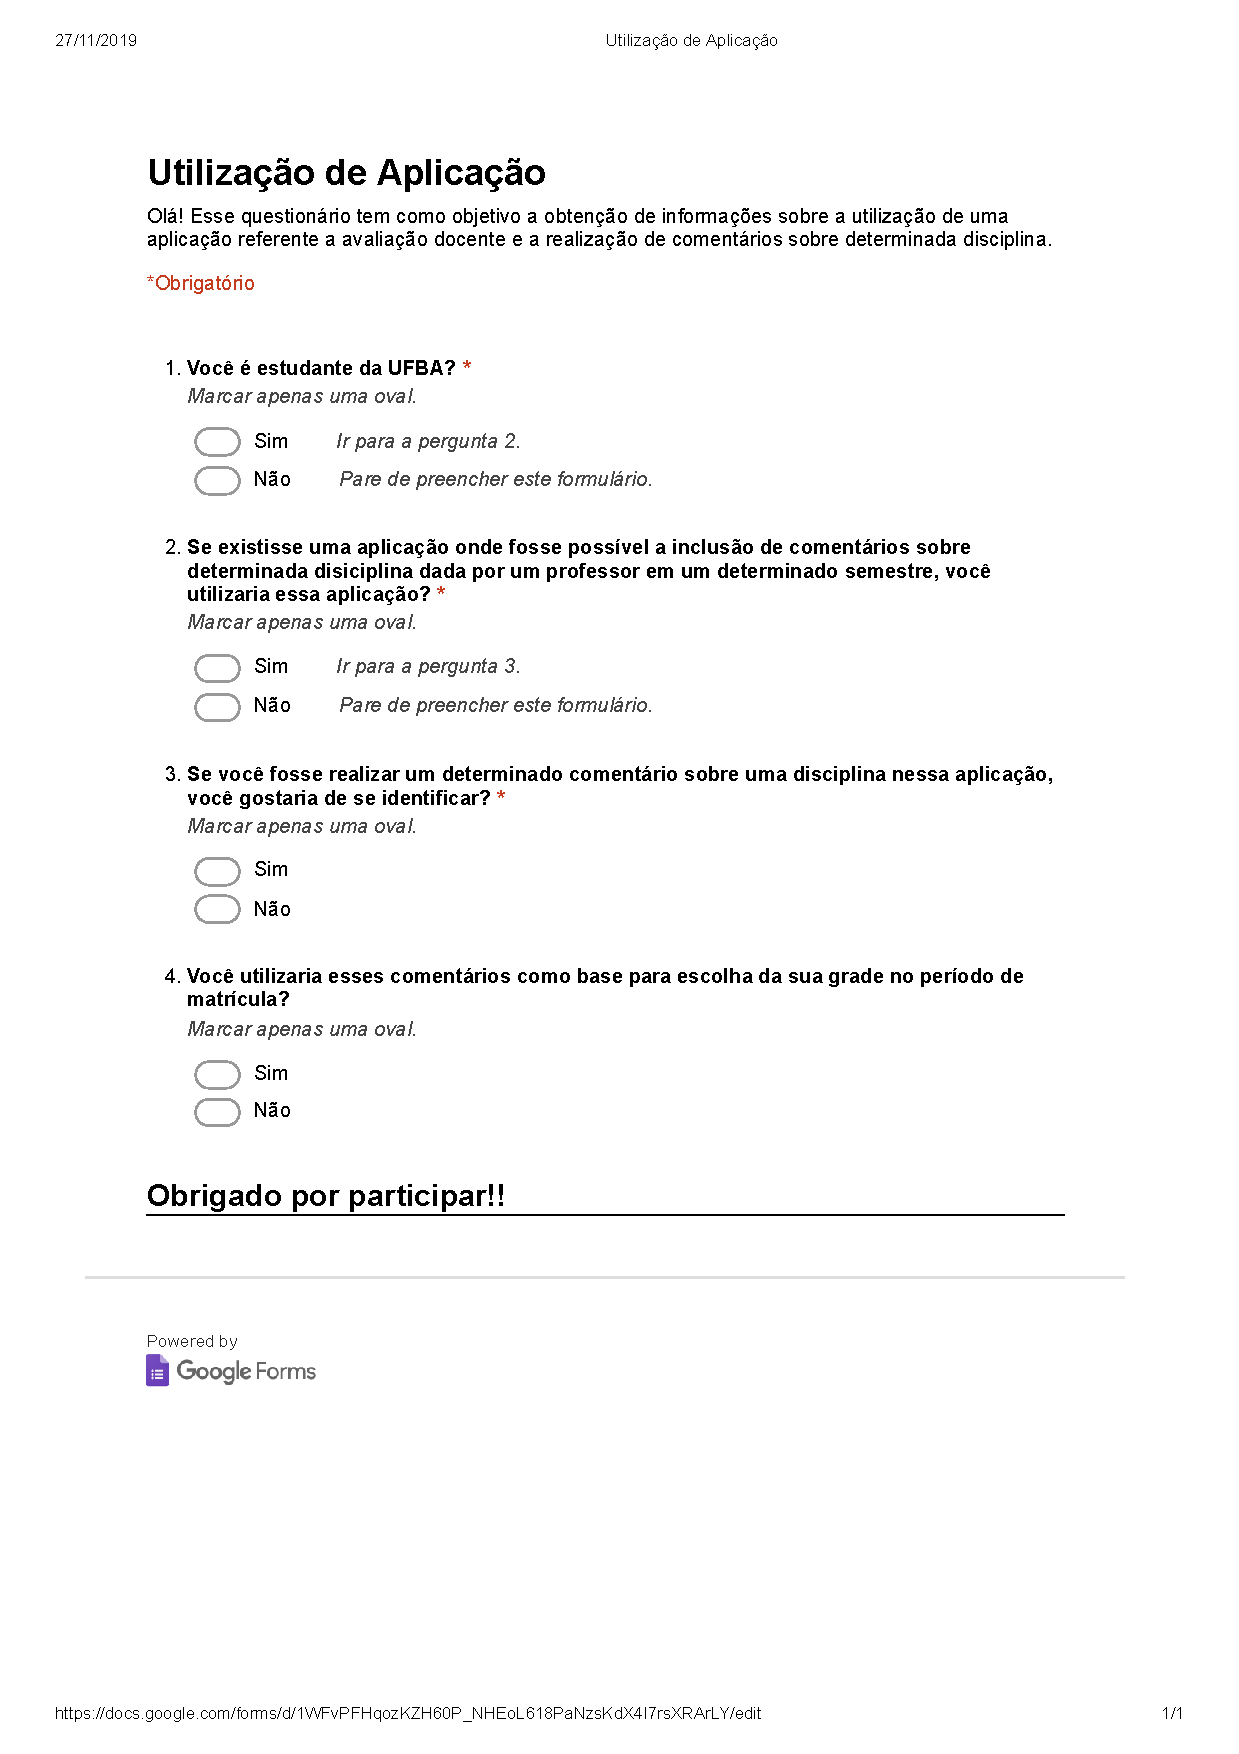
\includepdf[pages=-]{./formularios/SICAD.pdf}

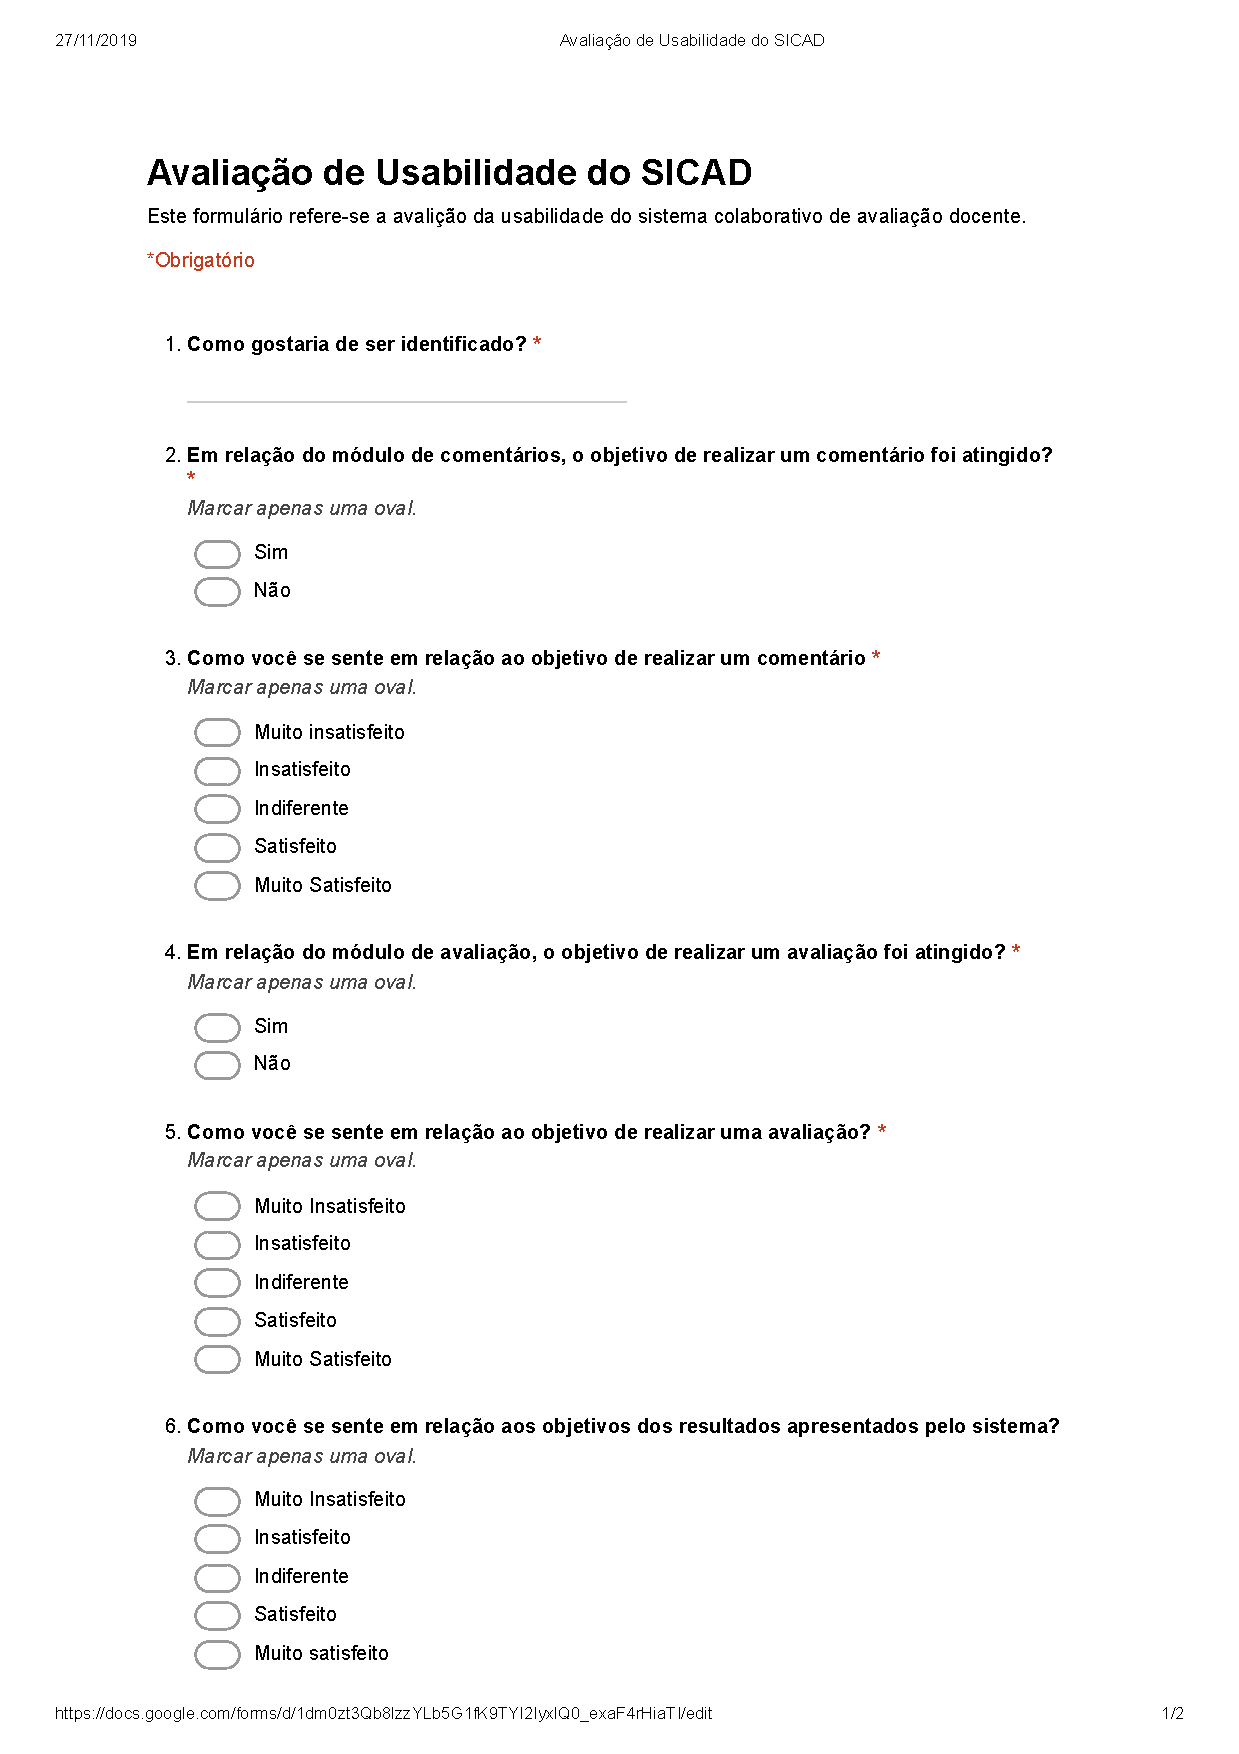
\includepdf[pages=-]{./formularios/Avaliacao.pdf}

\end{document}
